% Options for packages loaded elsewhere
\PassOptionsToPackage{unicode}{hyperref}
\PassOptionsToPackage{hyphens}{url}
%
\documentclass[
]{article}
\title{Weed community composition in simple and more diverse cropping systems}
\author{}
\date{\vspace{-2.5em}}

\usepackage{amsmath,amssymb}
\usepackage{lmodern}
\usepackage{iftex}
\ifPDFTeX
  \usepackage[T1]{fontenc}
  \usepackage[utf8]{inputenc}
  \usepackage{textcomp} % provide euro and other symbols
\else % if luatex or xetex
  \usepackage{unicode-math}
  \defaultfontfeatures{Scale=MatchLowercase}
  \defaultfontfeatures[\rmfamily]{Ligatures=TeX,Scale=1}
\fi
% Use upquote if available, for straight quotes in verbatim environments
\IfFileExists{upquote.sty}{\usepackage{upquote}}{}
\IfFileExists{microtype.sty}{% use microtype if available
  \usepackage[]{microtype}
  \UseMicrotypeSet[protrusion]{basicmath} % disable protrusion for tt fonts
}{}
\makeatletter
\@ifundefined{KOMAClassName}{% if non-KOMA class
  \IfFileExists{parskip.sty}{%
    \usepackage{parskip}
  }{% else
    \setlength{\parindent}{0pt}
    \setlength{\parskip}{6pt plus 2pt minus 1pt}}
}{% if KOMA class
  \KOMAoptions{parskip=half}}
\makeatother
\usepackage{xcolor}
\IfFileExists{xurl.sty}{\usepackage{xurl}}{} % add URL line breaks if available
\IfFileExists{bookmark.sty}{\usepackage{bookmark}}{\usepackage{hyperref}}
\hypersetup{
  pdftitle={Weed community composition in simple and more diverse cropping systems},
  hidelinks,
  pdfcreator={LaTeX via pandoc}}
\urlstyle{same} % disable monospaced font for URLs
\usepackage[margin=1in]{geometry}
\usepackage{longtable,booktabs,array}
\usepackage{calc} % for calculating minipage widths
% Correct order of tables after \paragraph or \subparagraph
\usepackage{etoolbox}
\makeatletter
\patchcmd\longtable{\par}{\if@noskipsec\mbox{}\fi\par}{}{}
\makeatother
% Allow footnotes in longtable head/foot
\IfFileExists{footnotehyper.sty}{\usepackage{footnotehyper}}{\usepackage{footnote}}
\makesavenoteenv{longtable}
\usepackage{graphicx}
\makeatletter
\def\maxwidth{\ifdim\Gin@nat@width>\linewidth\linewidth\else\Gin@nat@width\fi}
\def\maxheight{\ifdim\Gin@nat@height>\textheight\textheight\else\Gin@nat@height\fi}
\makeatother
% Scale images if necessary, so that they will not overflow the page
% margins by default, and it is still possible to overwrite the defaults
% using explicit options in \includegraphics[width, height, ...]{}
\setkeys{Gin}{width=\maxwidth,height=\maxheight,keepaspectratio}
% Set default figure placement to htbp
\makeatletter
\def\fps@figure{htbp}
\makeatother
\setlength{\emergencystretch}{3em} % prevent overfull lines
\providecommand{\tightlist}{%
  \setlength{\itemsep}{0pt}\setlength{\parskip}{0pt}}
\setcounter{secnumdepth}{-\maxdimen} % remove section numbering
\usepackage{lineno}
\linenumbers
\usepackage{float}
\usepackage{booktabs}
\usepackage{longtable}
\usepackage{array}
\usepackage{multirow}
\usepackage{wrapfig}
\usepackage{colortbl}
\usepackage{pdflscape}
\usepackage{tabu}
\usepackage{threeparttable}
\usepackage{threeparttablex}
\usepackage[normalem]{ulem}
\usepackage{makecell}
\usepackage{xcolor}
\setlength{\LTcapwidth}{\textwidth}
\ifLuaTeX
  \usepackage{selnolig}  % disable illegal ligatures
\fi
\usepackage[round]{natbib}
\bibliographystyle{plainnat}

\begin{document}
\maketitle

\hypertarget{abstract}{%
\section*{Abstract}\label{abstract}}
\addcontentsline{toc}{section}{Abstract}

Weed communities in three cropping systems suitable for the Midwestern USA were studied from 2017 through 2020 to examine how crop diversification and the intensity of herbicide use affected weed community diversity, stand density, and aboveground mass. A baseline 2-year cropping system with corn (\emph{Zea mays} L.) and soybean (\emph{Glycine max} (L.) Merr.) grown in alternate years was diversified with cool-season crops, namely oat (\emph{Avena sativa} L.), red clover (\emph{Trifolium pratense} L.), and alfalfa (\emph{Medicago sativa} L.) in 3-year and 4-year systems. Herbicide was not applied in the cool-season crops. Changing weed management regime from broadcast to banded application and interrow cultivation in corn and omitting herbicide in cool-season crops of the 3-year and 4-year rotations resulted in an overall reduction of herbicide a.i mass. The reduction in the mass of herbicide active ingredients was associated with increases in weed stand density, aboveground mass, and community diversity. Increased weed abundance under herbicide mass reduction was not associated with crop yield loss. In the cool-season crops phases of the 3-year and 4-year rotations, weed emergence was increased but weed growth was not, as compared with the warm-season crop environments. The dominance of aggressive weed species such as common waterhemp (\emph{Amaranthus tuberculatus} (Moq ex DC) J.D. Sauer) and common lambsquarter (\emph{Chenopodium album} L.) tended to be greater in corn and soybean phases of the rotations than in oat, red clover, and alfalfa.

\hypertarget{introduction}{%
\section*{Introduction}\label{introduction}}
\addcontentsline{toc}{section}{Introduction}

The composition of weed communities found in agricultural fields is strongly affected by the types of crops grown and their attendant management practices \citep{mohlerWeedEvolutionCommunity2001, legereDiversityAssemblyWeed2005, culpepperGlyphosateinducedWeedShifts2006, smithAssemblyWeedCommunities2007}. The US Corn Belt is dominated by monocultures and short-term rotations of corn and soybean \citep{centerforspatialinformationscienceandsystemsCropScapeCroplandData2021}. In response to simplified crop management customized for corn and soybean, weed communities have shifted to domination by aggressive summer annual species including common waterhemp (\emph{Amaranthus tuberculatus} (Moq ex DC) JD Sauer), Palmer amaranth (\emph{Amaranthus palmeri} S. Wats), giant ragweed (\emph{Ambrosia trifida} L.), common lambsquarter (\emph{Chenopodium album} L.), and woolly cupgrass (\emph{Eriochloa villosa} (Thunb) Kunth) \citep{owenWeedSpeciesShifts2008, krugerGrowerViewsProblematic2009, reddyGlyphosateresistantCropProduction2010}. Improved understanding of how management practices influence weed community composition could inform weed managers whether crop losses to weed competition are likely to occur and whether a weed community is shifting toward dominance by species that are more aggressive toward crops \citep{liebmanWeedManagementNeed2001}.

Cropping system diversification strategies that are designed to reduce reliance on external inputs, including herbicides, can balance productivity, profitability, and environmental quality goals \citep{davisIncreasingCroppingSystem2012, huntReducingFreshwaterToxicity2017, huntCroppingSystemDiversity2019, huntFossilEnergyUse2020, tamburiniAgriculturalDiversificationPromotes2020, bowlesLongtermEvidenceShows2020, beillouinPositiveVariableEffects2021}. They can also increase cropping systems' overall resilience to growing environmental adversity \citep{bowlesLongtermEvidenceShows2020} and can be effective in suppressing weeds \citep{weisbergerDoesDiversifyingCrop2019}. Increased crop species richness within crop sequences coupled with diversification of management practices applied to maximize crop and minimize weed resource acquisition, are expected to challenge weeds with large sets of stress and mortality factors compared to simple cropping systems \citep{liebmanManyLittleHammers1997, liebmanCropDiversificationWeed2001, westermanAreManyLittle2005}.

\citet{storkeyWhatGoodWeed2018} hypothesized that a more diverse weed community can be less competitive toward crops and weed seedbank diversity can be used as an indicator of cropping system sustainability. Nonetheless, few studies have examined weed community composition in rotations with crop species other than corn (\emph{Zea mays} L.), soybean (\emph{Glycine max} (L.) Merr.), and wheat (\emph{Triticum aestivum} L.), especially in fully phased settings, in which all crop phases within a rotation are present each year to control for year to year variations in weather conditions and management efficacy \citep{payneDesignAnalysisLong2015}. \citet{davisWeedSeedbankCommunity2005} studied weed aboveground and underground community shifts in four row-crop systems under four combinations of weed management and tillage regimes and found a strong negative relationship between crop yield and weed diversity, density, and total biomass; individual responses of only common waterhemp and common lambsquarter were reported. \citet{smithAssemblyWeedCommunities2007} compared a monoculture of corn with 2-year and 3-year rotations of corn with soybean and winter wheat, with or without cover crops and found that crop rotation and diversity had weak effects on weed community composition, whereas the cover crop in a particular rotation played an important role in weed species diversity. Increased reliance on glyphosate-based weed management has caused weed floras to shift to dominance by hard-to-control species \citep{owenWeedSpeciesShifts2008}, but it is unclear whether reduction in herbicide use would cause the same problem. \citet{liebmanWeedSeedbankDiversity2021} provided empirical evidence to support the hypothesis that seedbank diversity could be used as an indicator of cropping system sustainability \citet{storkeyWhatGoodWeed2018}.

This study was pursued to address the current gap of information concerning weed community density and aboveground mass responses to the filtering effects of different crop and weed management programs \citep{ryanManagementFiltersSpecies2010, friedTrajectoriesWeedCommunities2012}. We studied three different cropping systems suitable for the US Corn Belt. The baseline system was a conventional corn - soybean system. We diversified that baseline system with oat (\emph{Avena sativa} L.), red clover (\emph{Trifolium pratense} L.), and alfalfa (\emph{Medicago sativa} L.). Conventional broadcast herbicide and reduced herbicide management regimes were applied in a split-plot manner to corn phases of the three rotations. We hypothesized that diversified cropping systems, with reduced use of chemical herbicides, would provide weed control equal in effectiveness to the conventional approaches applied in the 2-year corn and soybean system. We assessed weed control efficacy by measuring weed aboveground mass and population densities. Additionally, we measured crop yields, positing that differences in weed aboveground mass and density could be reflected in differences in crop yields. Next, we hypothesized that the weed communities in the more diverse cropping systems would be more diverse, more even, and more species-rich than those in the 2-year corn and soybean system, reflecting a broader range of crop species and their attendant management practices in the more diverse rotations. Finally, we hypothesized that including oat, red clover, and alfalfa in rotations with corn and soybean would reduce the density and aboveground mass of noxious weed species in corn and soybean when the rotations cycles returned to corn and soybean.

\hypertarget{materials-and-methods}{%
\section*{Materials and Methods}\label{materials-and-methods}}
\addcontentsline{toc}{section}{Materials and Methods}

Empirical measurements of weed community composition were made from 2017 through 2020 at Iowa State University's Marsden Farm in Boone County, Iowa, USA, (42\(^\circ\) 01'N, 93\(^\circ\) 47'W, 333 m above sea level). All soil types present at the site are Mollisols \citep{chenInfluenceResidueNitrogen2014}. A detailed description of the experiment site and crop management can be found in \citet{liebmanWeedSeedbankDiversity2021} and the field layout and experiment design are provided in \citet{nguyenImpactCroppingSystemaccepted}. Briefly, a randomized complete block, split-plot design with four replications was used to study three different crop rotation systems (2-year, 3-year, or 4-year; the crop sequence in each rotation was presented in Table 1 of \citet{nguyenImpactCroppingSystemaccepted}). The main-plot factor, i.e., the crop identity, was represented by crop species and the rotation system in which it occurred (C2 - corn in the 2-year rotation, C3 - corn in the 3-year rotation, C4 - corn in the 4-year rotation, S2 - soybean in the 2-year rotation, S3 - soybean in the 3-year rotation, S4 - soybean in the 4-year rotation, O3 - oat in the 3-year rotation, and O4 - oat in the 4-year rotation, and A4 - alfalfa in the 4-year rotation). The split-plot factor, i.e., the weed management regime applied in the corn phase (corn weed management), was represented by herbicide level (conventional - pre- and post-emergent herbicides broadcast over the whole corn area, or low - post-emergence herbicides banded 38 cm wide on top of corn rows). The reduction of herbicide mass in the low herbicide treatment was supplemented by interrow cultivation. Details concerning crop genotypes and weed management regimes are provided in Table \ref{tab:herb-id}.

\begin{landscape}
\begin{ThreePartTable}
\begin{TableNotes}[para]
\item \textit{Note: } 
\item Corn was planted at 12950 seeds/ha, soybean at 56656 seeds/ha, oat at 80.7 kg/ha, red clover and alfalfa at 19.1 kg/ha. PRE and POST herbicide in corn and soybean refers to pre-emergence and post-emergence, relative to weed emergence. No herbicide was applied in oat, red clover, and alfalfa. 'Belle' (in 2017) or 'Mammoth' (in 2018 - 2020) red clover was intercropped with oat in the 3-year rotation (O3). Alfalfa was intercropped with the oat phase in the 4-year rotation (O4) and was overwintered to the following year as a sole crop (A4). Oat was replanted in 2020 due to poor germination.
\end{TableNotes}
\begin{longtable}[t]{>{\raggedright\arraybackslash}p{2em}>{\raggedright\arraybackslash}p{8em}>{\raggedright\arraybackslash}p{14em}>{\raggedright\arraybackslash}p{14em}>{\raggedright\arraybackslash}p{14em}>{\raggedright\arraybackslash}p{14em}}
\caption{\label{tab:herb-id}Crop variety or hybrid and management from 2017 through 2020 field seasons}\\
\toprule
\centering
Year & Activity or input & Low herbicide & Conventional herbicide & Low herbicide & Conventional herbicide\\
\midrule
\endfirsthead
\caption[]{\label{tab:herb-id}Crop variety or hybrid and management from 2017 through 2020 field seasons
\textit{(continued)}}\\
\toprule
\centering
Year & Activity or input & Low herbicide & Conventional herbicide & Low herbicide & Conventional herbicide\\
\midrule
\endhead

\endfoot
\bottomrule
\insertTableNotes
\endlastfoot
\textbf{} & \textbf{} & \textbf{Corn} & \textbf{Corn} & \textbf{Soybean} & \textbf{Soybean}\\
2017 & Hybrid or variety & Epley E1420 & Epley E1420 & Latham L2758 R2 & Latham L2758 R2\\
 & Planting date & 9-May & 9-May & 16-May & \\
 & Interrow cultivation date & Jun. 7 & Jun. 7 & none & none\\
 & Harvest date & Oct. 19 & Oct. 19 & Oct. 19 & \\
 & Herbicides applied (kg ai./ha) & POST: tembotrione (0.049) applied May 31, interrow cultivated Jun. 7 & PRE: thiencarbazone methyl (0.037), isoxaflutole (0.093) & PRE: flumioxazin (0.109); POST: glyphosate as potassium salt (1.249), acifluorfen (0.224) & PRE: flumioxazin (0.109); POST: glyphosate as potassium salt (1.249), acifluorfen (0.224)\\
 & Total (kg a.i./ha) & 0.049 & 0.13 & 1.581 & 1.581\\
 & Weed sampling date & Sep. 5 and 6 & Sep. 5 and 6 & Sep. 6, 7 and 8 & Sep. 6, 7 and 8\\
2018 & Hybrid or variety & Epley E1420 & Epley E1420 & Latham L2758 R2 & Latham L2758 R2\\
 & Planting date & 8-May & 8-May & Jun. 3 & Jun. 3\\
 & Interrow cultivation date & Jun. 4 & none & none & none\\
 & Harvest date & Oct. 30 & Oct. 30 & Oct. 29 & Oct. 29\\
 & Herbicides applied (kg ai./ha) & POST: tembotrione (0.054) & PRE: thiencarbazone methyl (0.037), isoxaflutole (0.092); POST: mesotrione (0.105), nicosulfuron (0.053) & PRE: flumioxazin (0.096); POST: glyphosate as potassium salt (1.540), lactofen (0.140) & PRE: flumioxazin (0.096); POST: glyphosate as potassium salt (1.540), lactofen (0.140)\\
 & Total (kg a.i./ha) & 0.054 & 0.287 & 1.776 & 1.776\\
 & Weed sampling date & Sep. 11, 12, and 13 & Sep. 11, 12, and 13 & Sep. 17, 19, 20, and 21 & Sep. 17, 19, 20, and 21\\
2019 & Hybrid or variety & Epley E1730 & Epley E1730 & Latham 2684 L (Liberty Link) & Latham 2684 L (Liberty Link)\\
 & Planting date & Jun. 3 & Jun. 3 & Jun. 10 & Jun. 10\\
 & Interrow cultivation date & none, due to weather adversity & none & none & none\\
 & Harvest date & Nov. 6 & Nov. 6 & Oct. 18 & Oct. 18\\
 & Herbicides applied (kg ai./ha) & POST: tembotrione (0.049) & PRE: thiencarbazone methyl (0.037), isoxaflutole (0.092); POST: mesotrione (0.105), nicosulfuron (0.053) & PRE: flumioxazin (0.096); POST: glufosinate ammonium (0.594), clethodim (0.136) & PRE: flumioxazin (0.096); POST: glufosinate ammonium (0.594), clethodim (0.136)\\
 & Total (kg a.i./ha) & 0.049 & 0.287 & 0.826 & 0.826\\
 & Weed sampling date & Sep. 17 and 18 & Sep. 17 and 18 & Sep. 30 & Sep. 30\\
2020 & Hybrid or variety & Epley E1730 & Epley E1730 & Latham 2684 L (Liberty Link) & Latham 2684 L (Liberty Link)\\
 & Planting date & Apr. 23 & Apr. 23 & 13-May & 13-May\\
 & Interrow cultivation date & Jun.8 & none & none & none\\
 & Harvest date & Oct. 2 & Oct. 2 & Sep. 23 & Sep. 23\\
 & Herbicides applied (kg ai./ha) & POST: tembotrione (0.051) & PRE: thiencarbazone methyl (0.037), isoxaflutole (0.092); POST: mesotrione (0.105), nicosulfuron (0.053) & PRE: flumioxazin (0.096); POST: glufosinate ammonium (0.594), clethodim (0.136) & PRE: flumioxazin (0.096); POST: glufosinate ammonium (0.594), clethodim (0.136)\\
 & Total (kg a.i./ha) & 0.051 & 0.287 & 0.826 & 0.826\\
 & Weed sampling date & Sep. 14 and 15 & Sep. 14 and 15 & Sep. 16 & Sep. 16\\
\textbf{} & \textbf{} & \textbf{Oat} & \textbf{Oat} & \textbf{Alfalfa} & \textbf{Alfalfa}\\
2017 & Hybrid or variety & IN09201 & IN09201 & Leafguard & Leafguard\\
 & Planting date & Apr. 12 & Apr. 12 & Mar. 29, 2016 & Mar. 29, 2016\\
 & Stubble clipping & Aug. 7 in O3 and O4 and Sep. 11 in O4 & Aug. 7 in O3 and O4 and Sep. 11 in O4 & Aug. 10, 2016 & Aug. 10, 2016\\
 & Harvest date & Jul. 17 & Jul. 17 & Jun.6, Jul. 7, Aug. 7, and Sep. 11 & Jun.6, Jul. 7, Aug. 7, and Sep. 11\\
 & Weed sampling date & Sep. 25, 27, 28 and 29 & Sep. 25, 27, 28 and 29 & Sep. 25, 27, 28 and 29 & Sep. 25, 27, 28 and 29\\
2018 & Hybrid or variety & IN09201 & IN09201 & Leafguard & Leafguard\\
 & Planting date & Apr. 24 & Apr. 24 & Apr. 12, 2017 & Apr. 12, 2017\\
 & Stubble clipping & Sep. 11 & Sep. 11 & Sep. 11, 2017 & Sep. 11, 2017\\
 & Harvest date & Jul. 20 & Jul. 20 & Jun. 4, Jul. 9, and Sep. 10 & Jun. 4, Jul. 9, and Sep. 10\\
 & Weed sampling date & Sep. 26, Oct.4, 15, 16, 18, and 19 & Sep. 26, Oct.4, 15, 16, 18, and 19 & Sep. 26, Oct.4, 15, 16, 18, and 19 & Sep. 26, Oct.4, 15, 16, 18, and 19\\
2019 & Hybrid or variety & IN09201 & IN09201 & Leafguard & Leafguard\\
 & Planting date & Apr. 16 & Apr. 16 & Apr. 24, 2018 & Apr. 24, 2018\\
 & Stubble clipping & none & none & none & \vphantom{1} none\\
 & Harvest date & Jul. 24 and 29 & Sep. 24 and 29 & Jun. 7, Jul. 12, Aug. 26, 2019 & Jun. 7, Jul. 12, Aug. 26, 2019\\
 & Weed sampling date & Sep. 23, 24, 25, and 26, Oct. 3, 4, 7, and 8 & Sep. 23, 24, 25, and 26, Oct. 3, 4, 7, and 8 & Sep. 23, 24, 25, and 26, Oct. 3, 4, 7, and 8 & Sep. 23, 24, 25, and 26, Oct. 3, 4, 7, and 8\\
2020 & Hybrid or variety & IN09201 & IN09201 & Leafguard & Leafguard\\
 & Planting date & Apr. 2, May 7 * & Apr. 2, May 7 * & Apr. 16, 2019 & Apr. 16, 2019\\
 & Stubble clipping & none & none & none & none\\
 & Harvest date & Jul. 24 & Jul. 24 & Jun. 2, Jul. 6, and Aug. 17 & Jun. 2, Jul. 6, and Aug. 17\\
 & Weed sampling date & Sep. 23, 24, and 29, Oct. 2, 6, 7, and 8 & Sep. 23, 24, and 29, Oct. 2, 6, 7, and 8 & Sep. 23, 24, and 29, Oct. 2, 6, 7, and 8 & Sep. 23, 24, and 29, Oct. 2, 6, 7, and 8\\*
\end{longtable}
\end{ThreePartTable}
\end{landscape}

Volunteer crops from a preceding crop season, such as a volunteer corn plant in a soybean plot or a soybean plant in an oat plot, were not considered weeds. Data were collected for individual weed species aboveground mass and density, community weed biomass and density, and crop yield. Weeds were surveyed four to six weeks before corn and soybean harvests, and two to three weeks after oat harvest or the last hay cut of the season.
The passage of a few weeks between oat and alfalfa harvest and weed surveys allowed physically damaged plants in those crops to grow back to recognizability. Weed aboveground samples were collected from eight quadrats arranged in a 4x2 grid throughout each experimental unit (eu). The sample grid was randomized every year in such a way that quadrats were at least 3 m away from plot borders to avoid any edge effect.

\hypertarget{individual-weed-species-abundance}{%
\paragraph*{Individual weed species abundance}\label{individual-weed-species-abundance}}
\addcontentsline{toc}{paragraph}{Individual weed species abundance}

All the same-species plants from each eu were clipped, enumerated, dried, and weighed at \textasciitilde0\% moisture together to make single data points per eu. The total surveyed area was 18.5 m\(^2\)/eu (8 x 2.3 m\(^2\)) in corn and soybean and 2.2 m\(^2\)/eu (8 x 0.28m\(^2\)) in oat and alfalfa. Plants were identified to species as guided by \citet{uvaWeedsNortheast1997}. Plant counts and dried weights were converted to plants m\(^{-2}\) and g m\(^{-2}\).

\hypertarget{weed-community-abundance}{%
\paragraph*{Weed community abundance}\label{weed-community-abundance}}
\addcontentsline{toc}{paragraph}{Weed community abundance}

Weights and counts of individual weed species from each eu were tallied for community abundance.

\hypertarget{ecological-indices}{%
\paragraph*{Ecological indices}\label{ecological-indices}}
\addcontentsline{toc}{paragraph}{Ecological indices}

Weed community diversity is the combination of two indices. The community evenness index ranges from 0 to 1, with higher values indicating higher evenness \citep{alataloProblemsMeasurementEvenness1981}. The species richness index is a count of the number of species observed. The presence of rare species in low abundance decreases the overall evenness of a weed community \citep{pielouInterpretationEcologicalData1984, stirlingEmpiricalRelationshipsSpecies2001}. Studying all three indices, i.e., diversity, evenness, and richness, generates a more complete description of a community than any one of the indices \citep{morrisChoosingUsingDiversity2014}. Simpson's diversity, evenness, and richness indices were calculated in terms of stand density and aboveground mass in each eu. We evaluated eighteen weed communities, corresponding to nine crop identities crossed with two weed management regimes in corn.

Let:\\
\(S\) represent species richness (i.e., the number of species presented),\\
\(n_i\) represent density of the i\(^{th}\) species (plants m\(^{-2}\)),\\
\(N\) represent density of all presented species (plants m\(^{-2}\)),\\
\(b_i\) represent aboveground mass of the i\(^{th}\) species (g m\(^{-2}\)),\\
\(B\) represent aboveground mass of all species, g m\(^{-2}\), and\\
\(p_{i_d}\) and \(p_{i_b}\) represent the proportional of density or aboveground biomass of the i\(^{th}\) species.

Community diversity was evaluated with Simpson's index, \(Simpson's\ D = \frac{1}{D} = \frac{1}{\sum p_i^2}\), because it is less sensitive to sample size and is useful to describe evenness \citep{nkoaWeedAbundanceDistribution2015}. Simpson's evenness index was calculated with \(\frac{\frac{1}{D}}{S}\). The \(p_i\) component in Simpson's diversity and evenness indices here was calculated with stand count (\(\frac{n_i}{N}\)) or biomass (\(\frac{b_i}{B}\)). Ideally, only one richness index is needed because it is the number of species presented. However, two ABUTH (\emph{Abutilon theophrasti}) plants that were found in 2019 were too light to register on a scientific scale, resulting in zero weight for the species' aboveground mass. Therefore, the richness index was calculated for both stand and aboveground mass. The evenness index was thus calculated with the relevant richness index with regards to stand count and aboveground mass.

\hypertarget{crop-yields}{%
\paragraph*{Crop yields}\label{crop-yields}}
\addcontentsline{toc}{paragraph}{Crop yields}

Six 84-m long rows of corn and soybean (383 m\(^2\)) were harvested from each eu, whereas for oat and alfalfa, whole plots were harvested (i.e., two adjacent subplots combined, 1530 m\(^2\)). Yields were adjusted to moisture concentrations of 155 g H\(_2\)O kg\(^{-1}\) for corn, 130 g H\(_2\)O kg\(^{-1}\) for soybean, 140 H\(_2\)O kg\(^{-1}\) for oat grain, and 150 g H\(_2\)O kg\(^{-1}\) for alfalfa.

\hypertarget{model-fitting}{%
\paragraph*{Model fitting}\label{model-fitting}}
\addcontentsline{toc}{paragraph}{Model fitting}

Block, crop identity, weed management regime applied to the corn phase of a rotation (corn weed management), and the interaction of crop identity and corn weed management were considered fixed factors; year and the interaction between year and the fixed factors were considered random factors; and the residual was random by default. Block was treated as a fixed factor to control for the different field conditions across sections and reduce the variance between eu's \citep{dixonShouldBlocksBe2016}.

R version 4.1.2 \citep{rdevelopmentcoreteamLanguageEnvironmentStatistical2021} was used for all data organization, manipulation, analysis, models diagnosis, and result presentation. Statistical tests were evaluated at an \(\alpha\) = 0.05 level of significance. All the response variables were natural logarithm (ln) transformed to ensure homogeneity of variance. For each response, the minimum non-zero value was added to zero values before transformation). Type III sums of squared error were calculated with the \texttt{emmeans} package's \texttt{joint\_tests} function to accommodate unbalanced data with interaction \citep[version 1.7.1-1,][]{lenthEmmeansEstimatedMarginal2021}. Results were back-transformed for presentation. Degree of freedom adjustment was done with Satterthwaite's method. P-values adjustment was done with Tukey's method.

Stand diversity, stand evenness, stand richness, aboveground mass diversity, aboveground mass evenness, aboveground mass richness, community aboveground density, community aboveground mass, individual species density, and individual species aboveground mass were analyzed separately with a linear mixed-effects model, using the \texttt{lmer} function in the \texttt{lme4} package \citep[version 1.1-27.1,][]{batesLme4LinearMixedEffects2021} according to the following model.

\begin{align}
R_{ijklm} = \mu + B_i + C_j + H_k + CH_{jk} + Y_l + BY_{il} + YC_{lj} + YH_{lk} + YCH_{ljk} + BYC_{ijl} + \epsilon_{ijkl}
\label{eq:index}
\end{align}

where,

\(R\) is one of the aforementioned responses,\\
\(\mu\) is the overall mean,\\
\(B\) is the block,\\
\(Y\) is the year,\\
\(C\) is the crop identity,\\
\(H\) is the corn weed management,\\
\(CH\) is the interaction between crop identity and corn weed management,\\
\(BY\) is the block within a year,\\
\(YC\) is interaction between crop identity and year,\\
\(YH\) is the interaction between year and corn herbicide,\\
\(YCH\) is the interaction between year, crop identity, and corn weed management,\\
\(BYC\) is the interaction between block, year, and crop identity, and\\
\(\epsilon_{ijklm}\) is the residual.

The crop identity term in the right-hand side of the model (Equation \eqref{eq:index}) represents the main-plot effect of the experiment, which comprises of the crop species and the rotation to which it belonged. In this present study, ``cropping system'' is the combination of ``rotation system'' (2-year, 3-year, and 4-year) and herbicide regime in corn (low or conventional); and crop type represents growing condition, so corn and soybean were grouped as warm-season crops, whereas oat and alfalfa were grouped as cool-season crops. With this model, we tested the following three sets of hypotheses for treatment effects on weed community stand diversity, community stand evenness, community stand richness, community aboveground mass diversity, community aboveground mass evenness, community aboveground mass richness, community aboveground density, and community aboveground mass:

\begin{enumerate}
\def\labelenumi{\arabic{enumi})}
\item
  The response variables increased as cropping system diversity increased.
\item
  In the same crop species the response variables differed between cropping systems.
\item
  In the same crop species the response variables differed between different crop types within a given cropping system.
\end{enumerate}

The first set of hypotheses was tested by contrasting the responses in the 2-year rotation with those in the average of the 3-year and 4-year rotations and the responses in the 3-year rotation with those in the 4-year rotation. The second set of hypotheses was tested by contrasting the responses in the same crop species within different rotations. The third set of hypotheses was tested by contrasting the average responses in the warm-season crops between rotations, in the cool-season crops between rotations, in the warm-season versus cool-season crops within the same rotation, and between the warm-season crops and the cool-season crop(s) averaged over rotations.

The same sets of contrasts used to evaluate weed community ecological indices, weed community aboveground mass, and weed community stand density were applied to data concerning the stand density and aboveground mass of the seven most abundant weed species to test for the treatment effects on those species:

\begin{enumerate}
\def\labelenumi{\arabic{enumi})}
\setcounter{enumi}{3}
\tightlist
\item
  The response variables differed between rotations for the same crop species, differed between rotations, and differed between crop type within a given cropping system.
\end{enumerate}

The fourth set of hypotheses was tested by contrasting individual weed species density and aboveground mass a) in the 2-year rotation versus the average of 3-year and 4-year rotations and in the 3-year versus 4-year rotation, b) in the same crop species or type between rotations, c) in different crop types within the same rotation, and d) in different crop types averaged over rotations.

A different linear mixed-effects model was used to analyze corn, soybean, and oat yields \citep[\texttt{lme4} version 1.1-27.1,][]{batesLme4LinearMixedEffects2021}:

\begin{align}
R_{ijkm} = \mu + B_i + C_j + H_k + CH_{jk} + Y_l + BY_{il} + YC_{lj} + YH_{lk}  + YRH_{lij} + BYC_{ilj} + \epsilon_{ijkl}
\label{eq:yield}
\end{align}

where,

\(R\) is the individual crop yield, and\\
all the terms in the right-hand side of the model are as defined in Equation \eqref{eq:index}.

As each crop species was fitted with a model, the crop identity represents the rotation effect only. With this model (Equation \eqref{eq:yield}), we tested the hypothesis that the yield of the same crop species (corn, soybean, and oat) did not differ between rotations. Crop yields were then contrasted between rotations to examine the magnitude of any significant difference.

\hypertarget{results}{%
\section*{Results}\label{results}}
\addcontentsline{toc}{section}{Results}

A lack of any obvious bias in plots of residuals versus predicted values suggested that the analysis models fit the data well. Diagnosis plots made with \texttt{ggResidpanel} \citep[version 0.3.0,][]{goodeGgResidpanelPanelsInteractive2019} are available in
\href{https://github.com/hnguyen19/Weed-community/blob/master/7-Extra/AppendixA-model-diagnosis.pdf}{Model Diagnosis}.


\hypertarget{how-did-rotation-system-and-corn-weed-management-affect-crop-yields}{%
\paragraph*{How did rotation system and corn weed management affect crop yields?}\label{how-did-rotation-system-and-corn-weed-management-affect-crop-yields}}
\addcontentsline{toc}{paragraph}{How did rotation system and corn weed management affect crop yields?}

Results of the experiment indicated that crop diversification and reduced use of herbicides were not associated with lower crop yields (Table \ref{tab:crop-jt-ct}). Averaged over four years, soybean was the only crop whose yield was affected by rotation (p = 0.0191, Table \ref{tab:crop-jt-ct}). Soybean yield was 16\% higher in the 4-year rotation than in the 2-year rotation (p = 0.0181). Crop yields in the experiment were as high or higher than the averages for the state of Iowa and Boone County (Figure \ref{fig:crop-bar}).

\begin{table}[H]

\caption{\label{tab:crop-jt-ct}Contrasts of rotation effect (expressed by Crop ID) on crop yields. The abbreviations on the contrast column are crop identities, which are the combinations of the first letter in crop species names and the rotation in which it occurred.}
\centering
\begin{threeparttable}
\begin{tabular}[t]{lrrr>{}r|lrr}
\toprule
\multicolumn{5}{c}{ANOVA} & \multicolumn{3}{c}{Comparison} \\
\cmidrule(l{3pt}r{3pt}){1-5} \cmidrule(l{3pt}r{3pt}){6-8}
Source of variation & df1 & df2 & F & p & contrast & ratio & p\\
\midrule
\addlinespace[0.3em]
\multicolumn{8}{l}{\textbf{(A) - Corn}}\\
\hspace{1em}Crop ID & 2 & 6 & 3.19 & 0.1138 & C2 vs C3 & 0.94 & 0.1882\\
\hspace{1em}Corn weed management & 1 & 3 & 0.32 & 0.6088 & C2 vs C4 & 0.93 & 0.1278\\
\hspace{1em}Crop ID x Corn weed management & 2 & 6 & 2.20 & 0.1914 & C3 vs C4 & 0.99 & 0.9507\\
\addlinespace[0.3em]
\multicolumn{8}{l}{\textbf{(B) - Soybean}}\\
\hspace{1em}Crop ID & 2 & 6 & 8.22 & 0.0191 & S2 vs S3 & 0.96 & 0.5499\\
\hspace{1em}Corn weed management & 1 & 3 & 0.18 & 0.7018 & S2 vs S4 & 0.86 & 0.0181\\
\hspace{1em}Crop ID x Corn weed management & 2 & 6 & 0.62 & 0.5677 & S3 vs S4 & 0.90 & 0.0670\\
\addlinespace[0.3em]
\multicolumn{8}{l}{\textbf{(C) - Oat}}\\
\hspace{1em}Crop ID & 1 & 2 & 1.14 & 0.3979 & O3 vs O4 & 0.91 & 0.3979\\
\bottomrule
\end{tabular}
\begin{tablenotes}[para]
\item \textit{Note: } 
\item Corn weed management: low herbicide or conventional. Crop ID: crop species and the cropping system in which it occurred: C2 - corn in the 2-year rotation, C3 - corn in the 3-year rotation, C4 - corn in the 4-year rotation, S2 - soybean in the 2-year rotation, S3 - soybean in the 3-year rotation, S4 - soybean in the 4-year rotation, O3 - oat in the 3-year rotation, and O4 - oat in the 4-year rotation.
\end{tablenotes}
\end{threeparttable}
\end{table}

\begin{figure}[H]
\centering
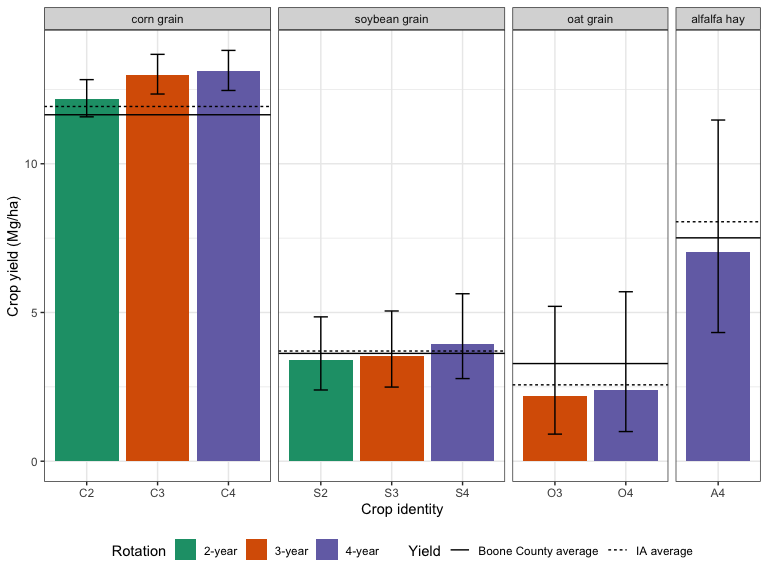
\includegraphics{crop-bar-1.png}
\caption{\label{fig:crop-bar}Mean crop yields by rotation from 2017 to 2020. The color-coded bars show crop yields (Mg ha\(^-1\)) in the experiment plots. The error bars show the 95\% confidence intervals. The solid horizontal lines show mean yields for Iowa and dashed lines show mean yields for Boone County. Corn, soybean, and alfalfa yields in the experiment were averaged over four years, oat grain yields in the experiment were averaged over 2017, 2019, and 2020 because in 2018 oat was harvested for hay. Boone County and Iowa hay yields were averaged over 2017 and 2018 because 2019 and 2020 yields were not available at this writing.}
\end{figure}

\hypertarget{how-did-rotation-system-crop-species-and-corn-weed-management-affect-community-ecological-indices}{%
\paragraph*{How did rotation system, crop species, and corn weed management affect community ecological indices?}\label{how-did-rotation-system-crop-species-and-corn-weed-management-affect-community-ecological-indices}}
\addcontentsline{toc}{paragraph}{How did rotation system, crop species, and corn weed management affect community ecological indices?}

Crop identity (i.e., rotation system x crop phase combination) affected weed community stand density evenness (p = 0.0064) and richness (p = 0.0123, Table \ref{tab:all-index-jt}C) and aboveground mass diversity (p = 0.0007, Table \ref{tab:all-index-jt}A), evenness (p = 0.0003, Table \ref{tab:all-index-jt}B), and richness (p =0.013). For all the differences in ecological indices, crop types were more influential than rotations, with larger differences found between crop types than between rotations (Figure \ref{fig:index-arrow-p}, Tables \ref{tab:dens-indices-ct} and \ref{tab:biom-indices-ct}).

\begin{table}[H]

\caption{\label{tab:all-index-jt}ANOVAs of crop identity, corn weed management, and their interactive effects on weed community ecological indices}
\centering
\begin{threeparttable}
\begin{tabular}[t]{lrrr>{}r|rr}
\toprule
\multicolumn{3}{c}{ } & \multicolumn{2}{c}{Stand density} & \multicolumn{2}{c}{Aboveground mass} \\
\cmidrule(l{3pt}r{3pt}){4-5} \cmidrule(l{3pt}r{3pt}){6-7}
Source of variation & df1 & df2 & F & p & F & p\\
\midrule
\addlinespace[0.3em]
\multicolumn{7}{l}{\textbf{(A) - Community diversity}}\\
\hspace{1em}Crop ID & 8 & 24 & 1.25 & 0.3116 & 5.22 & 0.0007\\
\hspace{1em}Corn weed management & 1 & 3 & 0.21 & 0.6804 & 0.47 & 0.5439\\
\hspace{1em}Crop ID x Corn weed management & 8 & 24 & 0.54 & 0.8182 & 1.35 & 0.2659\\
\addlinespace[0.3em]
\multicolumn{7}{l}{\textbf{(B) - Community evenness}}\\
\hspace{1em}Crop ID & 8 & 24 & 3.66 & 0.0064 & 5.87 & 0.0003\\
\hspace{1em}Corn weed management & 1 & 3 & 0.24 & 0.6589 & 0.01 & 0.9414\\
\hspace{1em}Crop ID x Corn weed management & 8 & 24 & 0.74 & 0.6547 & 0.47 & 0.8632\\
\addlinespace[0.3em]
\multicolumn{7}{l}{\textbf{(C) - Community richness}}\\
\hspace{1em}Crop ID & 8 & 24 & 3.23 & 0.0123 & 3.19 & 0.0130\\
\hspace{1em}Corn weed management & 1 & 3 & 1.32 & 0.3330 & 1.59 & 0.2959\\
\hspace{1em}Crop ID x Corn weed management & 8 & 24 & 0.71 & 0.6803 & 0.86 & 0.5635\\
\bottomrule
\end{tabular}
\begin{tablenotes}[para]
\item \textit{Note: } 
\item Corn weed management: low herbicide or conventional. Crop ID: crop species and the cropping system in which it occurred: C2 - corn in the 2-year rotation, C3 - corn in the 3-year rotation, C4 - corn in the 4-year rotation, S2 - soybean in the 2-year rotation, S3 - soybean in the 3-year rotation, S4 - soybean in the 4-year rotation, O3 - oat in the 3-year rotation, and O4 - oat in the 4-year rotation, and A4 - alfalfa in the 4-year rotation.
\end{tablenotes}
\end{threeparttable}
\end{table}

\begin{figure}[H]
\centering
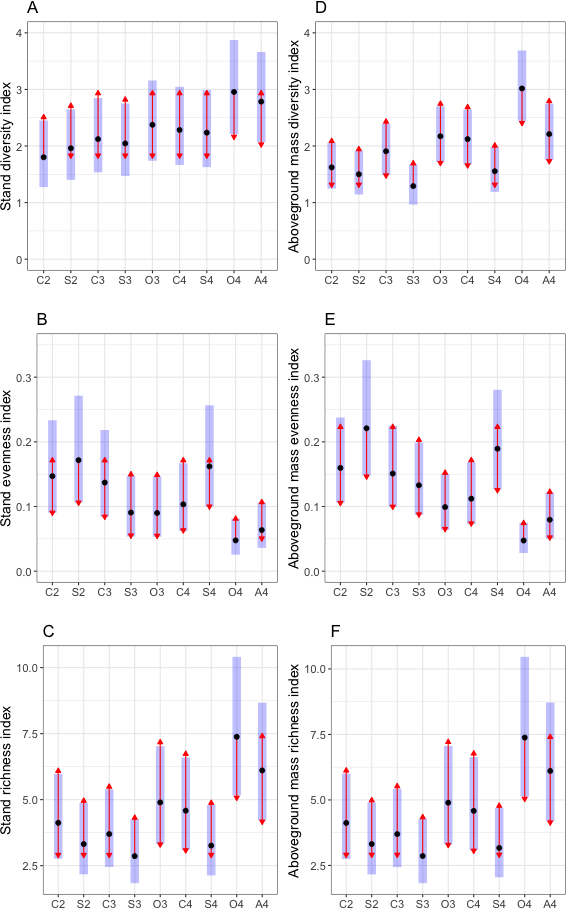
\includegraphics[width=.68\linewidth]{index-arrow-p-1.png}
\caption{\label{fig:index-arrow-p}Weed community stand diversity (A), evenness (B), and richness (C) and community aboveground diversity (D), evenness (E), and richness (F). The abbreviations on the x-axis are crop identities, which are the combinations of the first letter in crop species names and the rotation in which it occurred (C2 - corn in the 2-year rotation, C3 - corn in the 3-year rotation, C4 - corn in the 4-year rotation, S2 - soybean in the 2-year rotation, S3 - soybean in the 3-year rotation, S4 - soybean in the 4-year rotation, O3 - oat in the 3-year rotation, O4 - oat in the 4-year rotation, and A4 - alfalfa in the 4-year rotation). The black dots are estimated marginal means. The blue bars are 95\% confidence intervals. The red arrows reflect comparisons among means. Overlapping arrows indicate non-significant differences.}
\end{figure}

\emph{In general, the hypothesis that ``weed communities in the more diverse cropping systems are more diverse'' was supported.}

Averaged over crop phases within each rotation system (Table \ref{tab:dens-indices-ct}A), the weed community stand diversity index for the 3-year and 4-year rotation systems was comparable with that in the 2-year rotation (p = 0.0535 and p = 0.1575, respectively). For the individual crops (Table \ref{tab:dens-indices-ct}B), the weed stand density diversity index was comparable among rotations (p \textgreater{} 0.05). For different crop types (Table \ref{tab:dens-indices-ct}C), the weed community stand density diversity index in the average for the cool-season crops (O3, O4, and A4) was 1.2-fold greater than that in the average for the warm-season crops (C2, S2, C3, S3, C4, and S4) (p = 0.0145), but similar between the warm-season and cool-season crops in the same rotations (p = 0.4666 and p = 0.0987, respectively). The weed stand density diversity index was similar between oat and alfalfa (p = 0.7762).

Averaged over crop phases within the same rotation (Table \ref{tab:biom-indices-ct}A), the weed community aboveground mass diversity index was different between the 2-year rotation and the average of the 3-year and 4-year rotations (p = 0.0148), and between the 3-year and 4-year rotations (p = 0.0209). Averaged over the corn and soybean phases within the same rotation (Table \ref{tab:biom-indices-ct}A), the weed community aboveground mass diversity index was similar between rotations (p = 0.4217 and p = 0.2426, respectively). For the individual crops (Table \ref{tab:dens-indices-ct}B), the weed community aboveground mass diversity index was comparable between rotations, except for oat (p = 0.0351). For different crop types (Table \ref{tab:dens-indices-ct}C), the weed community aboveground mass diversity index in the cool-season crops average was 1.3-fold greater than that in the warm-season crops averages, overall (p \textless{} 0.0001), and was 1.23-fold and 1.27-fold greater in the cool-season than that in the warm-season crops in the 3-year (p = 0.034) and 4-year rotation (p = 0.0037), respectively. The weed community aboveground mass diversity index was comparable between oat and alfalfa (p = 0.2583).

\emph{The hypothesis that ``weed communities in the more diverse cropping systems are more even'' was partially supported (Figure \ref{fig:index-arrow-p}B and E).} However, a lower community evenness index can occur because the presence of rarer species decreases the overall evenness index \citep{stirlingEmpiricalRelationshipsSpecies2001}. More details to support this concept are presented later (Figure \ref{fig:all-sp-dens-biom}C and D).

Averaged over crop phases within the same rotation (Table \ref{tab:dens-indices-ct}A), the weed community stand density evenness index in the 2-year rotation was 1.6-fold greater than that in the average of the 3-year and 4-year rotations (p = 0.006), but comparable between the 3-year and 4-year rotations (p = 0.2802). Averaged over the corn and soybean phases within the same rotation (Table \ref{tab:dens-indices-ct}A), the weed community stand density evenness index was comparable between rotations (p = 0.1539 and p = 0.5031, respectively). For the individual crops (Table \ref{tab:dens-indices-ct}B), the weed community stand density evenness index was comparable between rotations (p \textgreater{} 0.05). For different crop types (Table \ref{tab:dens-indices-ct}C), the weed community stand density evenness index in the cool-season crops average was half of that in the warm-season crops average (p = 0.0002) and half of that in the cool-season and warm-season crop in the 4-year rotation (p = 0.0012), but similar between the warm-season and cool-season crops in the 3-year rotation (p = 0.4418). The weed community stand density evenness index was comparable between oat and alfalfa (p = 0.8986).

Averaged over crop phases within the same rotation (Table \ref{tab:biom-indices-ct}A), the weed community aboveground mass evenness index in the 2-year rotation was 1.65-fold greater than that in the average of 3-year and 4-year rotations (p = 0.0012), but similar between the 3-year and 4-year rotations (p = 0.0802). Averaged over the corn and soybean phases within the same rotation (Table \ref{tab:biom-indices-ct}A), weed community aboveground mass evenness index was comparable between rotations (p = 0.1081 and p = 0.8682, respectively). For the individual crops (Table \ref{tab:dens-indices-ct}B), the weed community aboveground mass evenness index was comparable between rotations (p \textgreater{} 0.05), except for oat (p = 0.0189). The weed community aboveground mass evenness index in the warm-season crops average was twice that of the cool-season crops average (p \textless{} 0.0001). The weed community aboveground mass evenness index in the warm-season crops was twice that of the cool-season crops in the 4-year rotation (p = 0.0002), but comparable between between the warm-season and cool-season crops in the 3-year rotation (p = 0.141), and between oat and alfalfa (p = 0.5911).

\emph{The hypothesis that ``the weed communities in the more diverse cropping systems are more species-rich'' was supported.}

Averaged over crop phases within the same rotation (Table \ref{tab:dens-indices-ct}A), the weed community stand density richness index was comparable in the 2-year rotation and in the average of the 3-year and 4-year rotations (p = 0.1819), but the stand density richness index in the 3-year was 0.77 that of the 4-year rotation (p = 0.0257). Averaged over the corn and soybean phases within the same rotation (Table \ref{tab:dens-indices-ct}A), weed community aboveground mass richness index was comparable between the 2-year rotation and the 3-year and 4-year rotations average (p = 0.7996) and between the 3-year and 4-year rotations (p = 0.3469). For individual crops (Table \ref{tab:dens-indices-ct}B), the weed community stand density richness index was comparable between rotations (p \textgreater{} 0.05). For different crop types (Table \ref{tab:dens-indices-ct}C), the weed stand density richness index in the cool-season crops average was 1.33-fold greater that of the warm-season crops average (p = 0.0003). Within the 4-year rotation, the weed stand density richness index in the cool-season was 1.58-fold greater than that in the warm-season crops (p = 0.0034). The weed stand density richness was comparable between the warm-season and cool-season crops in the 3-year rotation (p = 0.0725) and between oat and alfalfa (p = 0.9499).

The same patterns of difference and similarity of weed community richness index calculated with aboveground mass was observed (Table \ref{tab:biom-indices-ct}).

\begin{table}[H]

\caption{\label{tab:dens-indices-ct}Weed stand density ecological indices contrast significance. The abbreviations on the contrast column are crop identities, which are the combinations of the first letter in crop species names and the rotation in which it occurred.}
\centering
\begin{threeparttable}
\begin{tabular}[t]{lrrrlrr}
\toprule
\multicolumn{1}{c}{ } & \multicolumn{2}{c}{Diversity index} & \multicolumn{2}{c}{Evenness index} & \multicolumn{2}{c}{Richness index} \\
\cmidrule(l{3pt}r{3pt}){2-3} \cmidrule(l{3pt}r{3pt}){4-5} \cmidrule(l{3pt}r{3pt}){6-7}
Contrast & ratio & p & ratio & p & ratio & p\\
\midrule
\addlinespace[0.3em]
\multicolumn{7}{l}{\textbf{(A) - Rotation system effects}}\\
\hspace{1em}{}[(C2+S2)/2] vs [(C3+S3+O3+C4+S4+O4+A4)/7] & 0.85 & 0.0535 & 1.60 & 0.0060 & 0.86 & 0.1819\\
\hspace{1em}{}[(C3+S3+O3)/3] vs [(C4+S4+O4+A4)/4] & 0.90 & 0.1575 & 1.18 & 0.2802 & 0.77 & 0.0257\\
\hspace{1em}{}[(C2+S2)/2] vs [(C3+S3+C4+S4)/4] & 0.91 & 0.2749 & 1.28 & 0.1539 & 1.03 & 0.7996\\
\hspace{1em}{}[(C3+S3)/2] vs [(C4+S4)/2] & 0.95 & 0.5824 & 0.88 & 0.5031 & 0.87 & 0.3469\\
\addlinespace[0.3em]
\multicolumn{7}{l}{\textbf{(B) - Rotation system effects within individual crops}}\\
\hspace{1em}C2 vs [(C3+C4)/2] & 0.88 & 0.2836 & 1.20 & 0.4406 & 1.00 & 0.9985\\
\hspace{1em}C3 vs C4 & 0.95 & 0.7231 & 1.28 & 0.3757 & 0.84 & 0.3966\\
\hspace{1em}S2 vs [(S3+S4)/2] & 0.94 & 0.6331 & 1.36 & 0.2065 & 1.06 & 0.7212\\
\hspace{1em}S3 vs S4 & 0.94 & 0.6711 & 0.60 & 0.0746 & 0.91 & 0.6260\\
\hspace{1em}O3 vs O4 & 0.85 & 0.2716 & 1.66 & 0.0757 & 0.70 & 0.0912\\
\addlinespace[0.3em]
\multicolumn{7}{l}{\textbf{(C) - Crop type effects}}\\
\hspace{1em}{}[(O3+O4+A4)/3] vs [(C2+S2+C3+S3+C4+S4)/6] & 1.20 & 0.0145 & 0.55 & 0.0002 & 1.53 & 0.0003\\
\hspace{1em}O3 vs [(C3+S3)/2] & 1.09 & 0.4666 & 0.83 & 0.4418 & 1.38 & 0.0725\\
\hspace{1em}{}[(O4+A4)/2] vs [(C4+S4)/2] & 1.19 & 0.0987 & 0.49 & 0.0012 & 1.58 & 0.0034\\
\hspace{1em}{}[(O3+O4)/2] vs A4 & 0.97 & 0.7762 & 1.03 & 0.8986 & 0.99 & 0.9499\\
\bottomrule
\end{tabular}
\begin{tablenotes}[para]
\item \textit{Note: } 
\item C2 - corn in the 2-year rotation, C3 - corn in the 3-year rotation, C4 - corn in the 4-year rotation, S2 - soybean in the 2-year rotation, S3 - soybean in the 3-year rotation, S4 - soybean in the 4-year rotation, O3 - oat in the 3-year rotation, O4 - oat in the 4-year rotation, and A4 - alfalfa in the 4-year rotation
\end{tablenotes}
\end{threeparttable}
\end{table}

\begin{table}[H]

\caption{\label{tab:biom-indices-ct}Weed aboveground mass ecological indices contrast significance. The abbreviations on the contrast column are crop identities, which are the combinations of the first letter in crop species names and the rotation in which it occurred.}
\centering
\begin{threeparttable}
\begin{tabular}[t]{lrrrlrr}
\toprule
\multicolumn{1}{c}{ } & \multicolumn{2}{c}{Diversity index} & \multicolumn{2}{c}{Evenness index} & \multicolumn{2}{c}{Richness index} \\
\cmidrule(l{3pt}r{3pt}){2-3} \cmidrule(l{3pt}r{3pt}){4-5} \cmidrule(l{3pt}r{3pt}){6-7}
Contrast & ratio & p & ratio & p & ratio & p\\
\midrule
\addlinespace[0.3em]
\multicolumn{7}{l}{\textbf{(A) - Rotation system effects}}\\
\hspace{1em}{}[(C2+S2)/2] vs [(C3+S3+O3+C4+S4+O4+A4)/7] & 0.85 & 0.0148 & 1.65 & 0.0012 & 0.86 & 0.1967\\
\hspace{1em}{}[(C3+S3+O3)/3] vs [(C4+S4+O4+A4)/4] & 0.87 & 0.0209 & 1.27 & 0.0802 & 0.78 & 0.0309\\
\hspace{1em}{}[(C2+S2)/2] vs [(C3+S3+C4+S4)/4] & 0.95 & 0.4217 & 1.28 & 0.1081 & 1.04 & 0.7694\\
\hspace{1em}{}[(C3+S3)/2] vs [(C4+S4)/2] & 0.91 & 0.2426 & 0.97 & 0.8682 & 0.88 & 0.3930\\
\addlinespace[0.3em]
\multicolumn{7}{l}{\textbf{(B) - Rotation system effects within individual crops}}\\
\hspace{1em}C2 vs [(C3+C4)/2] & 0.87 & 0.1425 & 1.20 & 0.3825 & 1.00 & 0.9985\\
\hspace{1em}C3 vs C4 & 0.93 & 0.5084 & 1.31 & 0.2780 & 0.84 & 0.4035\\
\hspace{1em}S2 vs [(S3+S4)/2] & 1.03 & 0.7219 & 1.36 & 0.1543 & 1.08 & 0.6801\\
\hspace{1em}S3 vs S4 & 0.90 & 0.3166 & 0.72 & 0.1905 & 0.93 & 0.7075\\
\hspace{1em}O3 vs O4 & 0.79 & 0.0351 & 1.83 & 0.0189 & 0.70 & 0.0957\\
\addlinespace[0.3em]
\multicolumn{7}{l}{\textbf{(C) - Crop type effects}}\\
\hspace{1em}{}[(O3+O4+A4)/3] vs [(C2+S2+C3+S3+C4+S4)/6] & 1.30 & <.0001 & 0.51 & <.0001 & 1.54 & 0.0003\\
\hspace{1em}O3 vs [(C3+S3)/2] & 1.23 & 0.0340 & 0.73 & 0.1410 & 1.38 & 0.0766\\
\hspace{1em}{}[(O4+A4)/2] vs [(C4+S4)/2] & 1.27 & 0.0037 & 0.48 & 0.0002 & 1.60 & 0.0032\\
\hspace{1em}{}[(O3+O4)/2] vs A4 & 1.11 & 0.2583 & 0.89 & 0.5911 & 0.99 & 0.9506\\
\bottomrule
\end{tabular}
\begin{tablenotes}[para]
\item \textit{Note: } 
\item C2 - corn in the 2-year rotation, C3 - corn in the 3-year rotation, C4 - corn in the 4-year rotation, S2 - soybean in the 2-year rotation, S3 - soybean in the 3-year rotation, S4 - soybean in the 4-year rotation, O3 - oat in the 3-year rotation, O4 - oat in the 4-year rotation, and A4 - alfalfa in the 4-year rotation
\end{tablenotes}
\end{threeparttable}
\end{table}

\hypertarget{general-description-of-the-weed-flora}{%
\paragraph*{General description of the weed flora}\label{general-description-of-the-weed-flora}}
\addcontentsline{toc}{paragraph}{General description of the weed flora}

Overall, 34 weed species were identified during the four years of data collection (Table \ref{tab:list-sp}). Seven weed species, SETFA (\emph{Setaria faberi}), AMATA (\emph{Amaranthus tuberculatus}), CHEAL (\emph{Chenopodium album}), DIGSA (\emph{Digitaria sanguinalis}), ECHCG (\emph{Echinochloa crus-galli}), SETLU (\emph{Setaria glauca}), and TAROF (\emph{Taraxacum officinale}) made up 94.4\% of the total weed density and 94.0\% of the total weed biomass (Figure \ref{fig:all-sp-dens-biom}C and D).

\begin{table}[H]

\caption{\label{tab:list-sp}List of weed species (in alphabetical order) found from 2017 through 2020 field seasons.}
\centering
\begin{tabular}[t]{l|l|l}
\hline
Bayer code & Scientific name & Life cycle\\
\hline
\multicolumn{3}{l}{\textbf{(A) - Dicotyledon species}}\\
\hline
\hspace{1em}ABUTH & $Abutilon~theophrasti$$~$ Medicus & annual\\
 
\hspace{1em}AMARE & $Amaranthus~retrofelxus$$~$ L. & summer annual\\
 
\hspace{1em}AMATA & $Amaranthus~tuberculatus$$~$ (Moq.) Sauer~var.~$rudis$ & summer annual\\
 
\hspace{1em}AMBEL & $Ambrosia~artemissifolia$$~$ L. & erect, branching, summer annual\\
 
\hspace{1em}ARFMI & $Arctium~minus$$~$ (Hill) Bernh. & biennial\\
 
\hspace{1em}CHEAL & $Chenopodium~album$$~$ L. & erect summer annual\\
 
\hspace{1em}CIRAR & $Cirsium~arvense$$~$ (L.) Scop. & rhizomatous perennial\\
 
\hspace{1em}CIRVU & $Cirsium~vulgare$$~$ (Savi) Tenore & biennial\\
 
\hspace{1em}EPHHT & $Euphorbia~humistrata$$~$ Engelm.$~$ex$~$Gray & mat-forming summer annual\\
 
\hspace{1em}EPHMA & $Euphorbia~maculata$$~$ L. & mat-forming summer annual\\
 
\hspace{1em}EUPHY & $Eupatorium~hyssopifolium$$~$ L. & summer annual\\
 
\hspace{1em}MORAL & $Morus~alba$$~$ L. & perennial shrub\\
 
\hspace{1em}PHYSU & $Physalis~subglabrata$$~$ Mackenz. and Bush & rhizomatous perennial\\
 
\hspace{1em}PLAMA & $Plantago~major$$~$ L. & rosette-forming perennial\\
 
\hspace{1em}POLPE & $Polygonum~perfoliatum$$~$ L. & spiny summer annual vine\\
 
\hspace{1em}POLPY & $Polygonum~pensylvanicum$$~$ L. & ascending much-branched summer annual\\
 
\hspace{1em}POROL & $Portulaca~oleracea$$~$ L. & prostrate mat-forming summer annual\\
 
\hspace{1em}SOLPT & $Solanum~ptycanthum$$~$ Dun. & erect branching summer annual\\
 
\hspace{1em}SONAR & $Sonchus~arvensis$$~$ L. & rhizomatous perennial\\
 
\hspace{1em}TAROF & $Taraxacum~officinale$$~$Weberin$~$Wiggers & tap-rooted perennial\\
 
\multicolumn{3}{l}{\textbf{(B) - Monocotyledon species}}\\
\hline
\hspace{1em}AGRRE & $Elytrigia~repens$$~$ (L.) Nevski & rhizomatous perennial\\
 
\hspace{1em}BROTE & $Bromus~tectorum$$~$ L. & summer or winter annual\\
 
\hspace{1em}CCHPA & $Cenchrus~longispinus$$~$ (Hack.) Fern. & summer annual\\
 
\hspace{1em}CONAR & $Convolvulus~arvensis$$~$ L. & rhizomatous perennial\\
 
\hspace{1em}CYPES & $Cyperus~esculentus$$~$ L. & rhizomatous perennial\\
 
\hspace{1em}DACGL & $Dactylis~glomerata$$~$ L. & clump-forming perennial\\
 
\hspace{1em}DIGSA & $Digitaria~sanguinalis$$~$~(L.)~Scop. & summer annual\\
 
\hspace{1em}ECHCG & $Echinochloa~crus-galli$$~$ (L.) Beauv. & summer annual\\
 
\hspace{1em}ERBVI & $Eriochloa~villosa$$~$ (Thunb.) Kunth & erect summer annual\\
 
\hspace{1em}FESSP & $Festuca$$~$ spp. & clump-forming perennial\\
 
\hspace{1em}PANCA & $Panicum~capillare$$~$ L. & summer annual\\
 
\hspace{1em}PANDI & $Panicum~dichotomiflorum$$~$Michx. & summer annual\\
 
\hspace{1em}SETFA & $Setaria~faberi$$~$ Herrm. & clump-forming, erect summer annual\\
 
\hspace{1em}SETLU & $Setaria~glauca$$~$ (L.) Beauv. & clump-forming, erect summer annual\\
\hline
\end{tabular}
\end{table}

\hypertarget{how-did-rotation-crop-species-and-corn-weed-management-affect-weed-community-density-and-growth}{%
\paragraph*{How did rotation, crop species, and corn weed management affect weed community density and growth?}\label{how-did-rotation-crop-species-and-corn-weed-management-affect-weed-community-density-and-growth}}
\addcontentsline{toc}{paragraph}{How did rotation, crop species, and corn weed management affect weed community density and growth?}

Crop identity affected weed community stand density (p \textless{} 0.0001) and weed community aboveground mass (p = 0.0057), but corn weed management and its interaction with crop identity did not affect weed community stand density or biomass (p-values \textgreater{} 0.05) (Tables \ref{tab:dens-indices-ct} and \ref{tab:biom-indices-ct}). Weed community stand density and aboveground mass in each crop identity category, averaged over blocks, years, and corn weed management regimes, are presented in Figure \ref{fig:all-sp-dens-biom}A and B. Contributions by the dominant species are presented in Figure \ref{fig:all-sp-dens-biom}C and D. Contrasts for the effects of rotation systems, rotation system within individual crops, and crop types on community stand density and aboveground mass are shown in Table \ref{tab:dens-biom-jt-ct}C.

Weed community density and aboveground mass of the 3-year and 4-year systems averages were comparable to those of the 2-year system (p = 0.058 and p = 0.9451, respectively; Table \ref{tab:dens-biom-jt-ct}B1). The weed community density in the 4-year rotation was 2.5-fold greater than that in the 3-year rotation (p = 0.0368), but the community aboveground mass was comparable between the 3-year and 4-year rotations.

For the individual crops (Table \ref{tab:dens-biom-jt-ct}B2), increased rotation diversity tended to decrease weed density and aboveground mass in corn and soybean and increase weed abundance in oat, but these changes were not significant (p = 0.6354 and p = 0.4041 for corn, p = 0.1834 and p = 0.0739 for soybean, and p = 0.3955 and p = 0.335 for oat). The patchiness of weeds, which was reflected in the high standard error values, might have caused the lack of significance for these inconclusive trends.

For different crop types, weed community density and aboveground mass were comparable between the warm-season crops (corn and soybean) and between the cool-season crops (oat and alfalfa) (Table \ref{tab:dens-biom-jt-ct}B3). Overall, the average weed community density in the cool-season crops was 26-fold greater than that in the warm-season crops (p \textless{} 0.0001), and the average weed community aboveground mass in cool-season crops was 16-fold greater than that in warm-season crops (p = 0.0001). In the 3-year rotation, the weed stand community stand in oat (O3) was 11.5-fold greater than the average in corn and soybean (C3 and S3) (p = 0.0012), but the weed community aboveground mass was comparable between O3 and the average of the C3 and S3 phases (p = 0.1502). In the 4-year rotation, the weed community stand density in the average of oat and alfalfa (O4 and A4) was 36-fold greater than the average of the corn (C4) and soybean (S4) phases (p \textless{} 0.0001), and the average weed biomass for the O4 and A4 phases was 29-fold greater than that for the C4 and S4 phases (p \textless{} 0.0001).

\begin{table}[H]

\caption{\label{tab:dens-biom-jt-ct}Community density and aboveground mass ANOVA and contrasts. The abbreviations in the contrast column are crop identities, which are the combinations of the first letter in crop species names and the rotation in which it occurred.}
\centering
\begin{threeparttable}
\begin{tabular}[t]{lrrrrrr}
\toprule
\multicolumn{3}{c}{ } & \multicolumn{2}{c}{Stand density} & \multicolumn{2}{c}{Aboveground mass} \\
\cmidrule(l{3pt}r{3pt}){4-5} \cmidrule(l{3pt}r{3pt}){6-7}
Source of variation & df1 & df2 & F & p & F & p\\
\midrule
\addlinespace[0.3em]
\multicolumn{7}{l}{\textbf{(A) - ANOVA}}\\
\hspace{1em}Crop ID & 8 & 24 & 12.22 & <.0001 & 3.74 & 0.0057\\
 
\hspace{1em}Corn weed management & 1 & 3 & 2.13 & 0.2402 & 0.02 & 0.8900\\
 
\hspace{1em}Crop ID x Corn weed management & 8 & 24 & 1.66 & 0.1613 & 0.99 & 0.4660\\
 
\addlinespace[0.3em]
Contrasts  & & &               ratio & p & ratio  & p\\
\midrule
\addlinespace[0.3em]
\multicolumn{7}{l}{\textbf{(B1) - Rotation system effects}}\\
\hspace{1em}\hspace{1em}{}[(C2+S2)/2] vs [(C3+S3+O3+C4+S4+O4+A4)/7] &  &  & 0.42 & 0.0580 & 0.96 & 0.9451\\
 
\hspace{1em}\hspace{1em}{}[(C3+S3+O3)/3] vs [(C4+S4+O4+A4)/4] &  &  & 0.40 & 0.0368 & 0.42 & 0.1712\\
 
\addlinespace[0.3em]
\multicolumn{7}{l}{\textbf{(B2) - Rotation system effects within individual crops}}\\
\hspace{1em}\hspace{1em}C2 vs [(C3+C4)/2] &  &  & 1.38 & 0.6354 & 2.30 & 0.4041\\
 
\hspace{1em}\hspace{1em}C3 vs C4 &  &  & 0.59 & 0.4969 & 0.73 & 0.7853\\
 
\hspace{1em}\hspace{1em}S2 vs [(S3+S4)/2] &  &  & 2.49 & 0.1834 & 6.25 & 0.0739\\
 
\hspace{1em}\hspace{1em}S3 vs S4 &  &  & 1.19 & 0.8248 & 1.04 & 0.9731\\
 
\hspace{1em}\hspace{1em}O3 vs O4 &  &  & 0.51 & 0.3955 & 0.33 & 0.3350\\
 
\addlinespace[0.3em]
\multicolumn{7}{l}{\textbf{(B3) - Crop type effects}}\\
\hspace{1em}\hspace{1em}{}[(C2+S2)/2] vs [(C3+S3+C4+S4)/4] &  &  & 1.85 & 0.2032 & 3.79 & 0.0665\\
 
\hspace{1em}\hspace{1em}{}[(C3+S3)/2] vs [(C4+S4)/2] &  &  & 1.69 & 0.3426 & 3.54 & 0.1274\\
 
\hspace{1em}\hspace{1em}{}[(O3+O4+A4)/3] vs [(C2+S2+C3+S3+C4+S4)/6] &  &  & 26.10 & <.0001 & 16.00 & 0.0001\\
 
\hspace{1em}\hspace{1em}O3 vs [(C3+S3)/2] &  &  & 11.50 & 0.0012 & 4.29 & 0.1502\\
 
\hspace{1em}\hspace{1em}{}[(O4+A4)/2] vs [(C4+S4)/2] &  &  & 35.90 & <.0001 & 28.70 & 0.0003\\
 
\hspace{1em}\hspace{1em}{}[(O3+O4)/2] vs A4 &  &  & 0.80 & 0.7440 & 1.49 & 0.6870\\
\bottomrule
\end{tabular}
\begin{tablenotes}[para]
\item \textit{Note: } 
\item C2 - corn in the 2-year rotation, C3 - corn in the 3-year rotation, C4 - corn in the 4-year rotation, S2 - soybean in the 2-year rotation, S3 - soybean in the 3-year rotation, S4 - soybean in the 4-year rotation, O3 - oat in the 3-year rotation, O4 - oat in the 4-year rotation, and A4 - alfalfa in the 4-year rotation.
\end{tablenotes}
\end{threeparttable}
\end{table}

\begin{figure}[H]
\centering
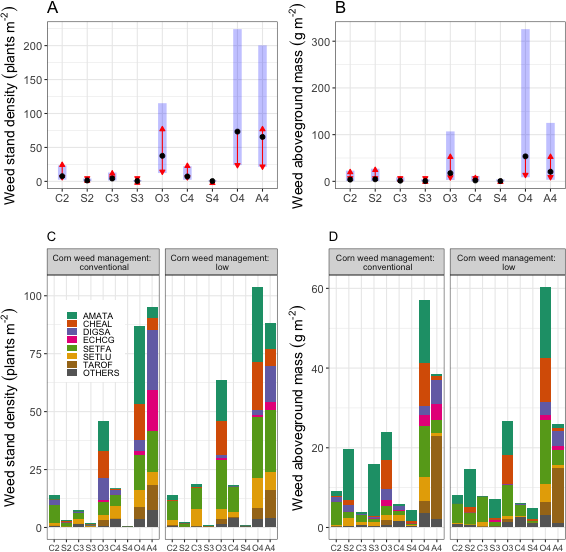
\includegraphics{all-sp-dens-biom-1.png}
\caption{\label{fig:all-sp-dens-biom}In panels A and B: weed community stand density and aboveground mass were averaged over four blocks, four years, and two corn weed management regimes; the black dots are estimated marginal means; the blue bars are 95\% confidence intervals; the red arrows reflect the comparisons among means; overlapping arrows indicate non-significant differences. In panels C and D: the contribution of the seven most abundant weed species and the rarer species (species ordered eighth and above grouped in OTHERS) in each crop identity, averaged over four blocks and four years, are ordered alphabetically. The abbreviations on the x-axis are crop identities, which are the combinations of the first letter in crop species names and the rotation in which it occurred (C2 - corn in the 2-year rotation, C3 - corn in the 3-year rotation, C4 - corn in the 4-year rotation, S2 - soybean in the 2-year rotation, S3 - soybean in the 3-year rotation, S4 - soybean in the 4-year rotation, O3 - oat in the 3-year rotation, O4 - oat in the 4-year rotation, and A4 - alfalfa in the 4-year rotation.) The less abundant weed species which made up 6\% of the whole community are grouped in OTHERS. The means displayed on panels A and B were estimated marginal means, calculated based on the analysis model (with \texttt{emmip} function) but the means displayed on panels C and D were arithmetic means, calculated from the data so they are slightly different.}
\end{figure}

\hypertarget{how-did-rotation-crop-species-and-corn-weed-management-affect-individual-weed-species-abundance}{%
\paragraph*{How did rotation, crop species, and corn weed management affect individual weed species abundance?}\label{how-did-rotation-crop-species-and-corn-weed-management-affect-individual-weed-species-abundance}}
\addcontentsline{toc}{paragraph}{How did rotation, crop species, and corn weed management affect individual weed species abundance?}  

\emph{The hypothesis that ``including oat and alfalfa in rotations with corn and soybean will reduce the density and aboveground mass of noxious weed species in corn and soybean'' was partially supported.} Crop identity affected individual density of seven most abundant weed species but corn weed management affected that of two weed species only, i.e., DIGSA and SETFA (p = 0.0189 and p = 0.0196, resepectively; Table \ref{tab:ind-dens-biom-jt}. Among those seven weed species, the aboveground mass of four (CHEAL, DIGSA, SETFA, and TAROF) were affected by crop identity, but none was affected by corn weed management (Table \ref{tab:ind-dens-biom-jt}). The magnitude of difference in stand density and aboveground mass were the most pronounced between crop types (Table \ref{tab:indiv-dens-biom-ct}). The main-plot effects concerning crop identity on individual species responses are elaborated below.

\begin{table}[H]

\caption{\label{tab:ind-dens-biom-jt}Treatment effects on the stand density and aboveground mass of the seven most abundant weed species, listed alphabetically. All the other weeds species were grouped into OTHERS.}
\centering
\resizebox{\linewidth}{!}{
\begin{threeparttable}
\begin{tabular}[t]{lrrr>{}r|rr}
\toprule
\multicolumn{3}{c}{ } & \multicolumn{2}{c}{Stand density} & \multicolumn{2}{c}{Aboveground mass} \\
\cmidrule(l{3pt}r{3pt}){4-5} \cmidrule(l{3pt}r{3pt}){6-7}
Source of variation & df1 & df2 & F & p & F & p\\
\midrule
\addlinespace[0.3em]
\multicolumn{7}{l}{\textbf{(A) - AMATA}}\\
\hspace{1em}Crop ID & 8 & 24 & 3.72 & 0.0058 & 1.52 & 0.2016\\
 
\hspace{1em}Corn weed management & 1 & 3 & 0.73 & 0.4566 & 4.19 & 0.1333\\
 
\hspace{1em}Crop ID x Corn weed management & 8 & 24 & 0.96 & 0.4886 & 1.09 & 0.4052\\
 
\addlinespace[0.3em]
\multicolumn{7}{l}{\textbf{(B) - CHEAL}}\\
\hspace{1em}Crop ID & 8 & 24 & 22.06 & <.0001 & 15.53 & <.0001\\
 
\hspace{1em}Corn weed management & 1 & 3 & 2.10 & 0.2430 & 0.56 & 0.5097\\
 
\hspace{1em}Crop ID x Corn weed management & 8 & 24 & 1.59 & 0.1808 & 1.07 & 0.4180\\
 
\addlinespace[0.3em]
\multicolumn{7}{l}{\textbf{(C) - DIGSA}}\\
\hspace{1em}Crop ID & 8 & 24 & 15.52 & <.0001 & 8.14 & <.0001\\
 
\hspace{1em}Corn weed management & 1 & 3 & 21.52 & 0.0189 & 16.44 & 0.0270\\
 
\hspace{1em}Crop ID x Corn weed management & 8 & 24 & 1.25 & 0.3126 & 0.78 & 0.6237\\
 
\addlinespace[0.3em]
\multicolumn{7}{l}{\textbf{(D) - ECHCG}}\\
\hspace{1em}Crop ID & 8 & 24 & 2.61 & 0.0328 & 2.20 & 0.0645\\
 
\hspace{1em}Corn weed management & 1 & 3 & 5.80 & 0.0952 & 4.84 & 0.1150\\
 
\hspace{1em}Crop ID x Corn weed management & 8 & 24 & 1.16 & 0.3615 & 1.04 & 0.4348\\
 
\addlinespace[0.3em]
\multicolumn{7}{l}{\textbf{(E) - SETFA}}\\
\hspace{1em}Crop ID & 8 & 24 & 8.78 & <.0001 & 4.22 & 0.0028\\
 
\hspace{1em}Corn weed management & 1 & 3 & 20.91 & 0.0196 & 13.96 & 0.0334\\
 
\hspace{1em}Crop ID x Corn weed management & 8 & 24 & 0.70 & 0.6892 & 1.04 & 0.4371\\
 
\addlinespace[0.3em]
\multicolumn{7}{l}{\textbf{(F) - SETLU}}\\
\hspace{1em}Crop ID & 8 & 24 & 3.09 & 0.0154 & 1.33 & 0.2774\\
 
\hspace{1em}Corn weed management & 1 & 3 & 4.44 & 0.1257 & 3.28 & 0.1681\\
 
\hspace{1em}Crop ID x Corn weed management & 8 & 24 & 1.11 & 0.3930 & 0.83 & 0.5875\\
 
\addlinespace[0.3em]
\multicolumn{7}{l}{\textbf{(G) - TAROF}}\\
\hspace{1em}Crop ID & 8 & 24 & 49.63 & <.0001 & 35.81 & <.0001\\
 
\hspace{1em}Corn weed management & 1 & 3 & 0.61 & 0.4914 & 0.33 & 0.6067\\
 
\hspace{1em}Crop ID x Corn weed management & 8 & 24 & 0.74 & 0.6553 & 1.20 & 0.3382\\
 
\addlinespace[0.3em]
\multicolumn{7}{l}{\textbf{(H) - OTHERS}}\\
\hspace{1em}Crop ID & 8 & 24 & 4.76 & 0.0014 & 2.35 & 0.0503\\
 
\hspace{1em}Corn weed management & 1 & 3 & 1.99 & 0.2533 & 2.27 & 0.2288\\
 
\hspace{1em}Crop ID x Corn weed management & 8 & 24 & 0.07 & 0.9997 & 0.43 & 0.8939\\
\bottomrule
\end{tabular}
\begin{tablenotes}[para]
\item \textit{Note: } 
\item Corn weed management: low herbicide or conventional. C2 - corn in the 2-year rotation, C3 - corn in the 3-year rotation, C4 - corn in the 4-year rotation, S2 - soybean in the 2-year rotation, S3 - soybean in the 3-year rotation, S4 - soybean in the 4-year rotation, O3 - oat in the 3-year rotation, O4 - oat in the 4-year rotation, and A4 - alfalfa in the 4-year rotation.
\end{tablenotes}
\end{threeparttable}}
\end{table}

\emph{The cool-season crops were responsible for AMATA stand density differences, but those differences were not strong enough to be apparent between rotation averages.} AMATA stand density and aboveground mass were comparable among all rotation systems averaged over crop phases (p-values \textgreater{} 0.05), among rotations for the same crop species (p-values \textgreater{} 0.05), and within the same crop type across rotations (p-values \textgreater{} 0.05). Averaged over the same crop types (warm-season or cool-season), AMATA stand density in cool-season was 12.25-fold greater than that in warm-season crops (p = 0.0001), but AMATA aboveground mass was comparable in cool-season and warm-season crops (p = 0.0906). Within the same rotation, AMATA stand density was 11-fold (p = 0.0143) and 23-fold (p = 0.0003) greater in the cool-season than in the warm-season crops overall averages, but AMATA aboveground mass was comparable in these crop environments (p = 0.2355 and p = 0.0493, respectively).

\emph{The cool-season crops, especially oat were responsible for CHEAL stand density and aboveground mass differences between rotation averages.} CHEAL stand density and aboveground mass were 4-fold (p = 0.008) and 5-fold (p = 0.199) greater in the average of the 3-year and 4-year rotations than in the 2-year rotation, but comparable between the 3-year and 4-year rotations (p = 0.9195 and p = 0.6114, respectively). CHEAL stand density and aboveground mass were comparable between rotations for the same crop species (p-values \textgreater{} 0.05) and within the warm-season crops (p-values \textgreater{} 0.05). CHEAL stand density and aboveground mass were 38-fold (p \textless{} 0.0001) and 204-fold (p \textless{} 0.0001) greater in the cool-season crops than in the warm-season crops overall averages; 67-fold (p \textless{} 0.0001) and 571-fold (p \textless{} 0.0001) greater in the cool-season crop than in the warm-season crops average of the 3-year rotation; and 37-fold (p \textless{} 0.0001) and 232-fold (p \textless{} 0.0001) greater in the cool-season crop than in the warm-season crops average of the 4-year rotation. CHEAL stand density and aboveground mass were 11-fold (p = 0.0001) and 96-fold (p = 0.0001) greater in oat than in alfalfa.

\emph{The cool-season crops, especially alfalfa were responsible for DIGSA stand density and aboveground mass differences between rotation averages.} DIGSA stand density in the average of the 3-year and 4-year rotations was two-fold greater than in the 2-year rotation (p = 0.0072) and 5-fold greater in the 4-year rotation than in the 3-year rotation (p \textless{} 0.0001). DIGSA aboveground mass was comparable between the 2-year and the average of the 3-year and 4-year rotations (p = 0.1098), but 14-fold greater in the 4-year than in the 3-year rotations (p = 0.0001). DIGSA stand density and aboveground mass were comparable between rotations for the same crop species (p-values \textgreater{} 0.05), except for oat (p = 0.0062 and p = 0.0032). DIGSA stand density and aboveground mass were 10-fold and 27-fold greater in the cool-season crop averages than in the warm-season crops averages, 20-fold (p = 0.0001) and 103-fold (p = 0.0001) greater in the cool-season crops than in the warm-season crops of the 4-year rotation, but comparable between cool-season and warm-season crops of the 3-year rotation (p = 0.0603 and p = 0.3924, respectively). DIGSA stand density and aboveground mass were 14-fold (p = 0.0001) and 33-fold (p = 0.0001) greater in alfalfa than in oat.

\emph{ECHCG responses generally were similar to those of AMATA.} ECHCG stand density and aboveground mass were comparable between all rotation averages (p-values \textgreater{} 0.05), between rotations for the same crop species (p-values \textgreater{} 0.05), within the same crop type between rotations (p-values \textgreater{} 0.05), and within the 3-year rotation (p-values \textgreater{} 0.05). Averaged over the same crop types, ECHCG stand density and aboveground mass were 4-fold (p = 0.0003) and 10-fold (p = 0.0012) greater in the cool-season than in the warm-season crops. Within the 4-year rotation, ECHCG stand density and aboveground mass were 5-fold (p = 0.0014) and 18-fold (p = 0.0031) greater in the cool-season than in the warm-season crops.

\emph{The cool-season crops were responsible for SETFA stand density and aboveground mass differences, but those differences were not strong enough be apparent between rotation averages.} SETFA stand density and aboveground mass were comparable between all rotation averages (p-values \textgreater{} 0.05), between rotations for the same crop species (p-values \textgreater{} 0.05), within the warm-season crops between rotations (p-values \textgreater{} 0.05), and within the cool-season crops (p-values \textgreater{} 0.05). Averaged over the same crop types, SETFA stand density and aboveground mass were 10-fold (p \textless{} 0.0001) and 15-fold (p = 0.0008) greater in the cool-season than in the warm-season crops. Within the same rotation, SETFA stand density and aboveground mass were 11-fold to 23-fold greater in the cool-season than in the warm-season crops (Table \ref{tab:indiv-dens-biom-ct}).

SETLU stand density and aboveground mass were comparable in most pairs of comparison (p-values \textgreater{} 0.05), except that SETLU stand density was 2.5-fold greater in the cool-season crops average than in the warm-season crops average(p = 0.0404).

\emph{The cool-season crops, especially oat were responsible for TAROF stand density and aboveground mass differences between rotation averages.} TAROF stand density and aboveground mass in the 3-year and 4-year rotations average were 4-fold (p \textless{} 0.0001) and 14-fold (p \textless{} 0.0001) greater than those in the 2-year rotation. TAROF stand density and aboveground mass in the 3-year rotation were and 5-fold (p \textless{} 0.0001) and 20-fold (p \textless{} 0.0001) greater than those in the 4-year rotation. TAROF stand density and aboveground mass were comparable among the warm-season crops between rotations and within the same crops between rotations (p-values \textgreater{} 0.05), except in oat (p \textless{} 0.0001). TAROF stand density and aboveground mass were 24-fold (p \textless{} 0.001) and 390-fold (p \textless{} 0.0001) greater in cool-season than in warm-season crop averages, 4-fold (p = 0.0001) and 20-fold (p = 0.0002) greater in oat than in corn and soybean averages in the 3-year rotation, and 54-fold (p \textless{} 0.0001) and 1483-fold (p \textless{} 0.0001) greater in the cool-season crops than in the warm-season crops in the 4-year rotation. TAROF stand density and aboveground mass were 6-fold (p \textless{} 0.0001) and 20-fold (p = 0.0001) greater in oat than in alfalfa.

\begin{landscape}\begin{table}[H]

\caption{\label{tab:indiv-dens-biom-ct}Contrast of stand density and aboveground mass of the seven most abundant weed species. Weed species are listed alphabetically. The abbreviations on the contrast column are crop identities, which are the combinations of the first letter in crop species names and the rotation in which it occurred.}
\centering
\resizebox{\linewidth}{!}{
\begin{threeparttable}
\begin{tabular}[t]{lr>{}r|r>{}r|r>{}r|r>{}r|r>{}r|r>{}r|rr}
\toprule
\multicolumn{1}{c}{ } & \multicolumn{2}{c}{AMATA} & \multicolumn{2}{c}{CHEAL} & \multicolumn{2}{c}{DIGSA} & \multicolumn{2}{c}{ECHCG} & \multicolumn{2}{c}{SETFA} & \multicolumn{2}{c}{SETLU} & \multicolumn{2}{c}{TAROF} \\
\cmidrule(l{3pt}r{3pt}){2-3} \cmidrule(l{3pt}r{3pt}){4-5} \cmidrule(l{3pt}r{3pt}){6-7} \cmidrule(l{3pt}r{3pt}){8-9} \cmidrule(l{3pt}r{3pt}){10-11} \cmidrule(l{3pt}r{3pt}){12-13} \cmidrule(l{3pt}r{3pt}){14-15}
Contrast of the main-plot effect & ratio & p & ratio & p & ratio & p & ratio & p & ratio & p & ratio & p & ratio & p\\
\midrule
\addlinespace[0.3em]
\multicolumn{15}{l}{\textbf{(A) - Stand density}}\\
\addlinespace[0.3em]
\multicolumn{15}{l}{\textbf{(A1) - Rotation system effects}}\\
\hspace{1em}\hspace{1em}{}[(C2+S2)/2] vs [(C3+S3+O3+C4+S4+O4+A4)/7] & 0.74 & 0.6105 & 0.28 & 0.0008 & 0.42 & 0.0072 & 0.57 & 0.1170 & 0.64 & 0.3011 & 0.50 & 0.1569 & 0.24 & <.0001\\
\hspace{1em}\hspace{1em}{}[(C3+S3+O3)/3] vs [(C4+S4+O4+A4)/4] & 0.81 & 0.7077 & 0.97 & 0.9195 & 0.21 & <.0001 & 0.55 & 0.0834 & 0.49 & 0.0927 & 0.44 & 0.0827 & 0.19 & <.0001\\
\hspace{1em}\hspace{1em}{}[(C2+S2)/2] vs [(C3+S3+C4+S4)/4] & 2.45 & 0.1746 & 1.37 & 0.3889 & 1.14 & 0.6798 & 0.98 & 0.9584 & 1.86 & 0.1906 & 0.70 & 0.4944 & 0.95 & 0.8129\\
\hspace{1em}\hspace{1em}{}[(C3+S3)/2] vs [(C4+S4)/2] & 1.76 & 0.4533 & 1.45 & 0.3823 & 0.69 & 0.3213 & 0.97 & 0.9384 & 0.75 & 0.5877 & 0.74 & 0.6234 & 0.84 & 0.5105\\
\addlinespace[0.3em]
\multicolumn{15}{l}{\textbf{(A2) - Rotation system effects within individual crops}}\\
\hspace{1em}\hspace{1em}C2 vs [(C3+C4)/2] & 2.33 & 0.3598 & 1.42 & 0.4995 & 0.93 & 0.8818 & 0.97 & 0.9497 & 1.56 & 0.5010 & 0.56 & 0.4277 & 1.02 & 0.9547\\
\hspace{1em}\hspace{1em}C3 vs C4 & 1.65 & 0.6368 & 1.31 & 0.6510 & 0.54 & 0.2466 & 0.89 & 0.8579 & 0.49 & 0.3501 & 0.49 & 0.3990 & 0.87 & 0.6923\\
\hspace{1em}\hspace{1em}S2 vs [(S3+S4)/2] & 2.58 & 0.3065 & 1.33 & 0.5837 & 1.40 & 0.4658 & 0.99 & 0.9915 & 2.21 & 0.2337 & 0.88 & 0.8628 & 0.88 & 0.6958\\
\hspace{1em}\hspace{1em}S3 vs S4 & 1.87 & 0.5543 & 1.60 & 0.4312 & 0.88 & 0.8088 & 1.04 & 0.9444 & 1.14 & 0.8620 & 1.14 & 0.8780 & 0.82 & 0.5914\\
\hspace{1em}\hspace{1em}O3 vs O4 & 0.32 & 0.2890 & 0.74 & 0.6212 & 0.21 & 0.0062 & 0.46 & 0.2130 & 0.59 & 0.4848 & 0.33 & 0.2006 & 0.09 & <.0001\\
\addlinespace[0.3em]
\multicolumn{15}{l}{\textbf{(A3) - Crop type effects}}\\
\hspace{1em}\hspace{1em}{}[(O3+O4+A4)/3] vs [(C2+S2+C3+S3+C4+S4)/6] & 12.25 & 0.0001 & 38.15 & <.0001 & 10.11 & <.0001 & 3.60 & 0.0003 & 9.85 & <.0001 & 2.48 & 0.0404 & 24.33 & <.0001\\
\hspace{1em}\hspace{1em}O3 vs [(C3+S3)/2] & 10.94 & 0.0143 & 67.07 & <.0001 & 2.43 & 0.0630 & 1.94 & 0.2248 & 11.32 & 0.0010 & 1.05 & 0.9435 & 4.33 & 0.0001\\
\hspace{1em}\hspace{1em}{}[(O4+A4)/2] vs [(C4+S4)/2] & 23.36 & 0.0003 & 36.99 & <.0001 & 20.08 & <.0001 & 4.82 & 0.0014 & 11.63 & 0.0001 & 2.96 & 0.0798 & 53.81 & <.0001\\
\hspace{1em}\hspace{1em}{}[(O3+O4)/2] vs A4 & 3.71 & 0.1606 & 10.75 & 0.0001 & 0.07 & <.0001 & 0.49 & 0.1954 & 1.17 & 0.8068 & 0.37 & 0.1812 & 0.17 & <.0001\\
\addlinespace[0.3em]
\multicolumn{15}{l}{\textbf{(B) - Aboveground mass}}\\
\addlinespace[0.3em]
\multicolumn{15}{l}{\textbf{(B1) - Rotation system effects}}\\
\hspace{1em}\hspace{1em}{}[(C2+S2)/2] vs [(C3+S3+O3+C4+S4+O4+A4)/7] & 3.10 & 0.3402 & 0.21 & 0.0199 & 0.36 & 0.1098 & 0.35 & 0.1417 & 0.93 & 0.9245 & 0.46 & 0.3588 & 0.07 & <.0001\\
\hspace{1em}\hspace{1em}{}[(C3+S3+O3)/3] vs [(C4+S4+O4+A4)/4] & 1.30 & 0.8168 & 1.33 & 0.6414 & 0.07 & 0.0001 & 0.32 & 0.1040 & 0.56 & 0.4497 & 0.39 & 0.2420 & 0.05 & <.0001\\
\hspace{1em}\hspace{1em}{}[(C2+S2)/2] vs [(C3+S3+C4+S4)/4] & 9.26 & 0.0893 & 2.30 & 0.2315 & 1.60 & 0.4852 & 0.89 & 0.8841 & 3.54 & 0.1566 & 0.58 & 0.5502 & 0.86 & 0.7608\\
\hspace{1em}\hspace{1em}{}[(C3+S3)/2] vs [(C4+S4)/2] & 2.83 & 0.4799 & 2.43 & 0.2676 & 0.54 & 0.4264 & 1.00 & 0.9958 & 0.94 & 0.9537 & 0.89 & 0.9148 & 0.67 & 0.4810\\
\addlinespace[0.3em]
\multicolumn{15}{l}{\textbf{(B2) - Rotation system effects within individual crops}}\\
\hspace{1em}\hspace{1em}C2 vs [(C3+C4)/2] & 7.45 & 0.2696 & 2.21 & 0.4167 & 1.06 & 0.9499 & 1.02 & 0.9882 & 2.81 & 0.4070 & 0.48 & 0.5668 & 0.94 & 0.9237\\
\hspace{1em}\hspace{1em}C3 vs C4 & 1.78 & 0.7802 & 1.70 & 0.6372 & 0.40 & 0.3994 & 0.69 & 0.7630 & 0.39 & 0.5131 & 0.50 & 0.6404 & 0.85 & 0.8309\\
\hspace{1em}\hspace{1em}S2 vs [(S3+S4)/2] & 11.50 & 0.1821 & 2.39 & 0.3720 & 2.40 & 0.3571 & 0.79 & 0.8252 & 4.47 & 0.2329 & 0.71 & 0.7847 & 0.80 & 0.7378\\
\hspace{1em}\hspace{1em}S3 vs S4 & 4.50 & 0.4709 & 3.49 & 0.2708 & 0.73 & 0.7772 & 1.44 & 0.7687 & 2.27 & 0.5667 & 1.59 & 0.7516 & 0.54 & 0.4336\\
\hspace{1em}\hspace{1em}O3 vs O4 & 0.14 & 0.3486 & 0.53 & 0.5666 & 0.03 & 0.0032 & 0.10 & 0.0768 & 0.29 & 0.3941 & 0.12 & 0.1539 & 0.01 & <.0001\\
\addlinespace[0.3em]
\multicolumn{15}{l}{\textbf{(B3) - Crop type effects}}\\
\hspace{1em}\hspace{1em}{}[(O3+O4+A4)/3] vs [(C2+S2+C3+S3+C4+S4)/6] & 6.11 & 0.0906 & 204.44 & <.0001 & 27.29 & <.0001 & 9.56 & 0.0012 & 15.00 & 0.0008 & 2.05 & 0.3316 & 389.81 & <.0001\\
\hspace{1em}\hspace{1em}O3 vs [(C3+S3)/2] & 8.70 & 0.2355 & 571.14 & <.0001 & 2.26 & 0.3924 & 2.54 & 0.3920 & 22.34 & 0.0180 & 0.47 & 0.5554 & 19.10 & 0.0002\\
\hspace{1em}\hspace{1em}{}[(O4+A4)/2] vs [(C4+S4)/2] & 20.20 & 0.0493 & 231.64 & <.0001 & 102.80 & <.0001 & 17.54 & 0.0031 & 22.79 & 0.0045 & 3.18 & 0.2706 & 1482.81 & <.0001\\
\hspace{1em}\hspace{1em}{}[(O3+O4)/2] vs A4 & 28.24 & 0.0724 & 94.46 & 0.0001 & 0.03 & 0.0008 & 0.64 & 0.6762 & 5.38 & 0.1818 & 0.43 & 0.5132 & 0.05 & 0.0001\\
\bottomrule
\end{tabular}
\begin{tablenotes}[para]
\item \textit{Note: } 
\item C2 - corn in the 2-year rotation, C3 - corn in the 3-year rotation, C4 - corn in the 4-year rotation, S2 - soybean in the 2-year rotation, S3 - soybean in the 3-year rotation, S4 - soybean in the 4-year rotation, O3 - oat in the 3-year rotation, O4 - oat in the 4-year rotation, and A4 - alfalfa in the 4-year rotation.
\end{tablenotes}
\end{threeparttable}}
\end{table}
\end{landscape}

\hypertarget{discussion}{%
\section*{Discussion}\label{discussion}}
\addcontentsline{toc}{section}{Discussion}

Diversification of cropping systems led to increased weed community aboveground mass and stand density, increased weed community diversity and species richness, and decreased weed community evenness. Increased weed abundance was not associated with reduced crop yield. Crop identity in the present experiment had the strongest influence on the response variables. This observation is consistent with previous studies in which crop identity showed the strongest influence on weed community characteristics \citep{legereDiversityAssemblyWeed2005, smithAssemblyWeedCommunities2007}. The observation that crop yields were not correlated with increased weed aboveground mass suggests that low amounts of weed biomass can be tolerated, rather than the commonly desired weed-free condition \citep{zimdahlNeedHistoricalPerspective2012}. Tolerating greater weed abundance can create some risks of resurgence by formerly prevalent weed species or outbreak of highly adapted introduced species under favorable conditions \citep{mohlerWeedEvolutionCommunity2001}. Consequently, weed growth and weed community composition should be monitored frequently to keep weed infestations at tolerable levels and to detect risks for future seasons. As weeds develop resistance to herbicides, weed eradication is likely to be increasingly impractical for technical, financial, and environmental reasons \citep{brookesKeyEnvironmentalImpacts2013, stewartWeedControlEnvironmental2011}, making the monitoring of weed communities a critically important component of weed management.

\citet{ryanManagementFiltersSpecies2010} found that weeds growing in a preceding crop phase of a sequence affected the subsequent seedbank more strongly than the seedbank influenced the emerged weed flora; the investigators attributed this a filtering effect of crop management on weed seed production by mixed-species communities. The four years of data presented here did not reveal any weed species that might become aggressive in the presence of oat, red clover, and alfalfa. Following the critical period for weed control concepts described by \citet{knezevicCriticalPeriodWeed2002}, weed control measures were applied in corn and soybean at their early establishment stages, but were not necessary in oat's early establishment because the most abundant weed species in this experiment site were summer annuals, whose emergence and establishment are synchronized with corn and soybean. Planting oat and red clover after soybean (in the 3-year rotation), instead of circling back to corn (as in the 2-year rotation), disrupted life cycles of those summer annual weeds. An extended disruption was also imposed in the 4-year rotation with the oat/alfalfa intercrop in year three and established alfalfa in year four. Frequent hay cuts severely suppressed weed species with erect stature, such as AMATA, CHEAL, and ECHCG, but did not significantly affect other species such as TAROF, SETFA, and SETLU. TAROF is a low stature weed, which was not as severely suppressed in alfalfa and oat as were AMATA, CHEAL, and ECHCG. SETFA and SETLU are clump-forming species that are less likely to be affected by harvest machinery. In oat, AMATA, CHEAL, ECHCG, SETFA, and SETLU, like most of the summer annual weeds at the experiment site, were in their early vegetative stages at oat harvest \citep{buhlerEmergencePersistenceSeed2001, cordeauHowWeedsDiffer2017}. By the weed sampling dates, those weeds were physically severed once by the oat harvest combine, or twice by additional stubble clipping if the weed pressure was deemed high.

Tolerating higher amount of weeds might increase the risk of crop damage if weeds can serve as alternative hosts to pathogens \citep{wislerInteractionsWeedsCultivated2005, mohlerCropDiseasePathogens2009}. However, soybean sudden death syndrome (SDS), caused by the soil-borne pathogen \emph{Fusarium virguliforme} \citep{hartmanResearchAdvancesManagement2015}, had its incidence and severity reduced due to cropping system diversification within the present experiment \citep{leandroCroppingSystemDiversification2018}. Among the currently recognized \emph{Fusarium virguliforme} alternative hosts that were present at the experiment site, crops, such as alfalfa and red clover are considered symptomatic while weeds such as lambsquarter and pigweed asymptomatic \citep{kolanderSymptomaticAsymptomaticHost2012}. Taking the findings of \citet{kolanderSymptomaticAsymptomaticHost2012} and \citet{leandroCroppingSystemDiversification2018} together, it is more likely that crops played more important roles than weeds in SDS outbreaks and that cropping system diversification can control the risk of SDS outbreak effectively.

Differences in weed responses to cropping systems and management practices were more pronounced in aboveground mass than in stand density (Tables \ref{tab:dens-indices-ct} and \ref{tab:biom-indices-ct}), which implied that rotation significantly affected weed growth but not weed emergence. These observations matched the general pattern reported by \citet{weisbergerDoesDiversifyingCrop2019}. We attributed the observed community composition shift to the differences in crop phenology and required management practices between the warm-season crops (corn and soybean) and the cool-season crops (oat and alfalfa) \citep{gabaAgroecologicalWeedControl2014, weisbergerDoesDiversifyingCrop2019}. In the present study, the magnitude of difference in sowing dates between soybean and oat seeded with red clover or alfalfa (60 days), as compared to that of corn and soybean (14 days), could be the largest contributor to reductions of weed density.

We considered the weed management programs in the 3-year and 4-year rotations effective because the crop yields at our experiment site were comparable between rotations (Table \ref{tab:crop-jt-ct}) and to averages for the state of Iowa and Boone County (Figure \ref{fig:crop-bar}). In the 2-year rotation, the net saved amount of herbicide between the low and conventional herbicide regimes was 13\% as soybean plots were all treated with conventional weed management practices. The mass of herbicide active ingredients was reduced further in the 3-year and 4-year rotations as corn and soybean were supplemented with oat, red clover, and alfalfa. For example, a 3-year rotation with corn under the low herbicide regime saved 42\% of herbicide active ingredients as compared to the 2-year rotation with corn under conventional weed management; and the 4-year rotation with corn under low herbicide weed management saved 57\% of herbicide active ingredients as compared to the 2-year rotation with corn under conventional weed management. We also considered two weed management programs for the same crop equally effective because the crop yields were not significantly different between corn weed management regimes. In the corn phase of the rotation systems, a transition from conventional to low herbicide weed management reduced the mass of herbicide active ingredients by 80\% over four years because herbicide was applied in a band half of the area planted to corn.

Weed community aboveground mass composition and individual aboveground mass responses to cropping system diversification suggested that the weed communities that were dominated by few competitive species in the corn and soybean phases of the 2-year rotation could be shifted to have more of the rarer, less aggressive species. Community shifts to rarer, less aggressive weed species were reflected in the significant differences in ecological indices between cool-season and warm-season crops. The reduction of herbicide use, especially during oat and alfalfa phases of the rotation allowed some rarer species to grow, and thus, higher species richness and lower evenness were observed in oat and alfalfa than in corn and soybean. Community evenness indices in warm-season crops were higher than those in cool-season crops because fewer weed species were found in corn and soybean. The experimental units with high evenness index values had species of similar abundance and competitiveness, such as AMATA and CHEAL. Although an even weed community is desirable because of reduced chances that one or a few species are dominantly competitive \citep{adeuxMitigatingCropYield2019}, weed communities could also be evenly dominated by a few weed species like AMATA, with high competitiveness, high reproduction potential, and quick herbicide resistance development. Thus, careful monitoring is required.

It is noteworthy that the relative abundance of the top seven species appeared more even in oat and alfalfa than in corn and soybean (Figure \ref{fig:all-sp-dens-biom}). Weeds can emerge in pulses in response to changes in soil conditions (e.g., temperature and moisture), so emergence after weed control measures have been applied and any residual effects have dissipated could result in successful establishment. Among the seven most abundant species in this experiment, five were influenced more strongly by crop identity than by corn weed management (Table \ref{tab:ind-dens-biom-jt}). This observation is consistent with previous findings that emphasized the role of crops in weed community shifts \citep{davisWeedSeedbankCommunity2005, smithAssemblyWeedCommunities2007, owenWeedSpeciesShifts2008, friedTrajectoriesWeedCommunities2012}.

Due to labor constraints, only eight quadrats were evaluated per experimental unit (eu), and the samples in the eight quadrats within the same eu were tallied to make one data point. By using Simpson's ecological indices, we have limited the sensitivity of the responses to sample size \citep{nkoaWeedAbundanceDistribution2015}. With eight quadrats randomly spaced within an eu, we sought to control for the patchiness of weed communities \citep{cardinaNatureConsequenceWeed1997}, but the list of weed species presented in this manuscript is likely to not be exhaustive of species at the experiment site. We suggest, however, that the responses of dominant weed species, which are more agronomically important than the rarer species, were representatively assessed because the effects of spatially separated blocks on responses were non-significant. Also due to labor constraints, individual plant weight was not assessed, so we could not explore how community evenness was affected by individual plant size and whether there was any relationship or coincidence between evenness and individual plant reproductive potential.

A community that is dominated by AMATA, CHEAL, DIGSA, ECHCG, SETFA, and SETLU is more concerning than one dominated by TAROF, as determined by the frequency that those species are regarded as problematic \citep{krugerGrowerViewsProblematic2009, princeBenchmarkStudyIntroduction2012}, their seedbank persistence characteristics \citep{buhlerEmergencePersistenceSeed2001, davisEnvironmentalFactorsAffecting2005}, and their invulnerability to the strongest control measures \citep{mohlerWeedEvolutionCommunity2001, culpepperGlyphosateinducedWeedShifts2006}. Further investigation of AMATA, CHEAL, DIGSA, ECHCG, SETFA, and SETLU population dynamics, including emergence patterns, survival throughout crop season, and reproductive potentials under various cropping systems could help guide efforts to regulate the timing of their emergence, limit their growth and reproductive potentials, and eventually deplete their seedbanks. The reproductive potential of AMATA was reduced substantially in cool-season crops as compared to warm-season crops \citep{nguyenImpactCroppingSystemaccepted}. Taking the finding of Nguyen and Liebman with those of \citet{gabaAgroecologicalWeedControl2014} and \citet{weisbergerDoesDiversifyingCrop2019}, it is likely that the cool-season crops in the present study served to deplete the soil seedbank by inducing seed loss through weed emergence and granivore activities \citep{vanderlaatPostdispersalWeedSeed2015}, while reducing reproduction potential through growth suppression. As demonstrated for SETFA \citep{davisCroppingSystemEffects2003a}, retrospective analyses applied to aggressive weed species can contribute to understanding species responses to management practices and to tailoring management tactics and timing to target them.

Overall, we conclude that by monitoring aboveground weed communities, a track record of species aggressiveness and collective response to management is available, and thus, it could be easier to control risks of weed resurgence and outbreak. Coupling knowledge of aboveground weed communities with that of weed seedbank composition and abundance would further improve our ability to predict and manage weed communities \citep{forcellaWeedSeedbanksCorn1992, menalledWeedAbovegroundSeedbank2001, forcellaDebitingSeedbankPriorities2003, davisWeedSeedbankCommunity2005}.

\hypertarget{acknowledgements}{%
\section*{Acknowledgements}\label{acknowledgements}}
\addcontentsline{toc}{section}{Acknowledgements}

The authors thank Matt Woods, Mike Fiscus, and the Iowa State University's Agronomy Research Farm crew for field management; Wendy Borja-Diaz, Lydia English, Jessica Juarez-Morales, Samantha Kanselaar, Jessica Nelson, Elizabeth Oys, Ana Poznanski, Andrew Riehl, Angela Soto-Saenz, Mickala Stallman, David Weisberger, and Wyatt Westfall for field and laboratory assistance; Katherine Goode, Audrey McCombs, Philip Dixon and ISU's statistical consulting group for data analysis assistance; Russ Lenth and other Stackoverflow community members for answering HTXN's coding questions; Micheal Owen for reviewing the manuscript; Overleaf staff for \LaTeX~assistance in compiling the manuscript; and two anonymous reviewers for their constructive feedback.

\renewcommand\refname{References}
  \bibliography{ecol.bib}

\end{document}
